\chapter{Methodology, Design and\\ Implementation}\label{chap:Methodology}

%Report and methodology section: note that the methodology of the signal processing is similar to the work that we covered in the audio radar course that showed how to get to the range-Doppler map. However, the methodology of your project should also include the design of the system, hardware choices, embedded processing choices, and signal processing aspects of the project. 

The methodology followed to design and test the implemented radar follows the V-Model shown in Figure \ref{V-Model}. The system would be broken down into sections and subsystems and tested individually before the integration of the system. Finally, the system as a whole would undergo acceptance testing per the user- and functional requirements and technical specifications. The requirements and specifications can be viewed in Section \ref{UserReqs}.

\begin{figure}[h!]
    \centering
    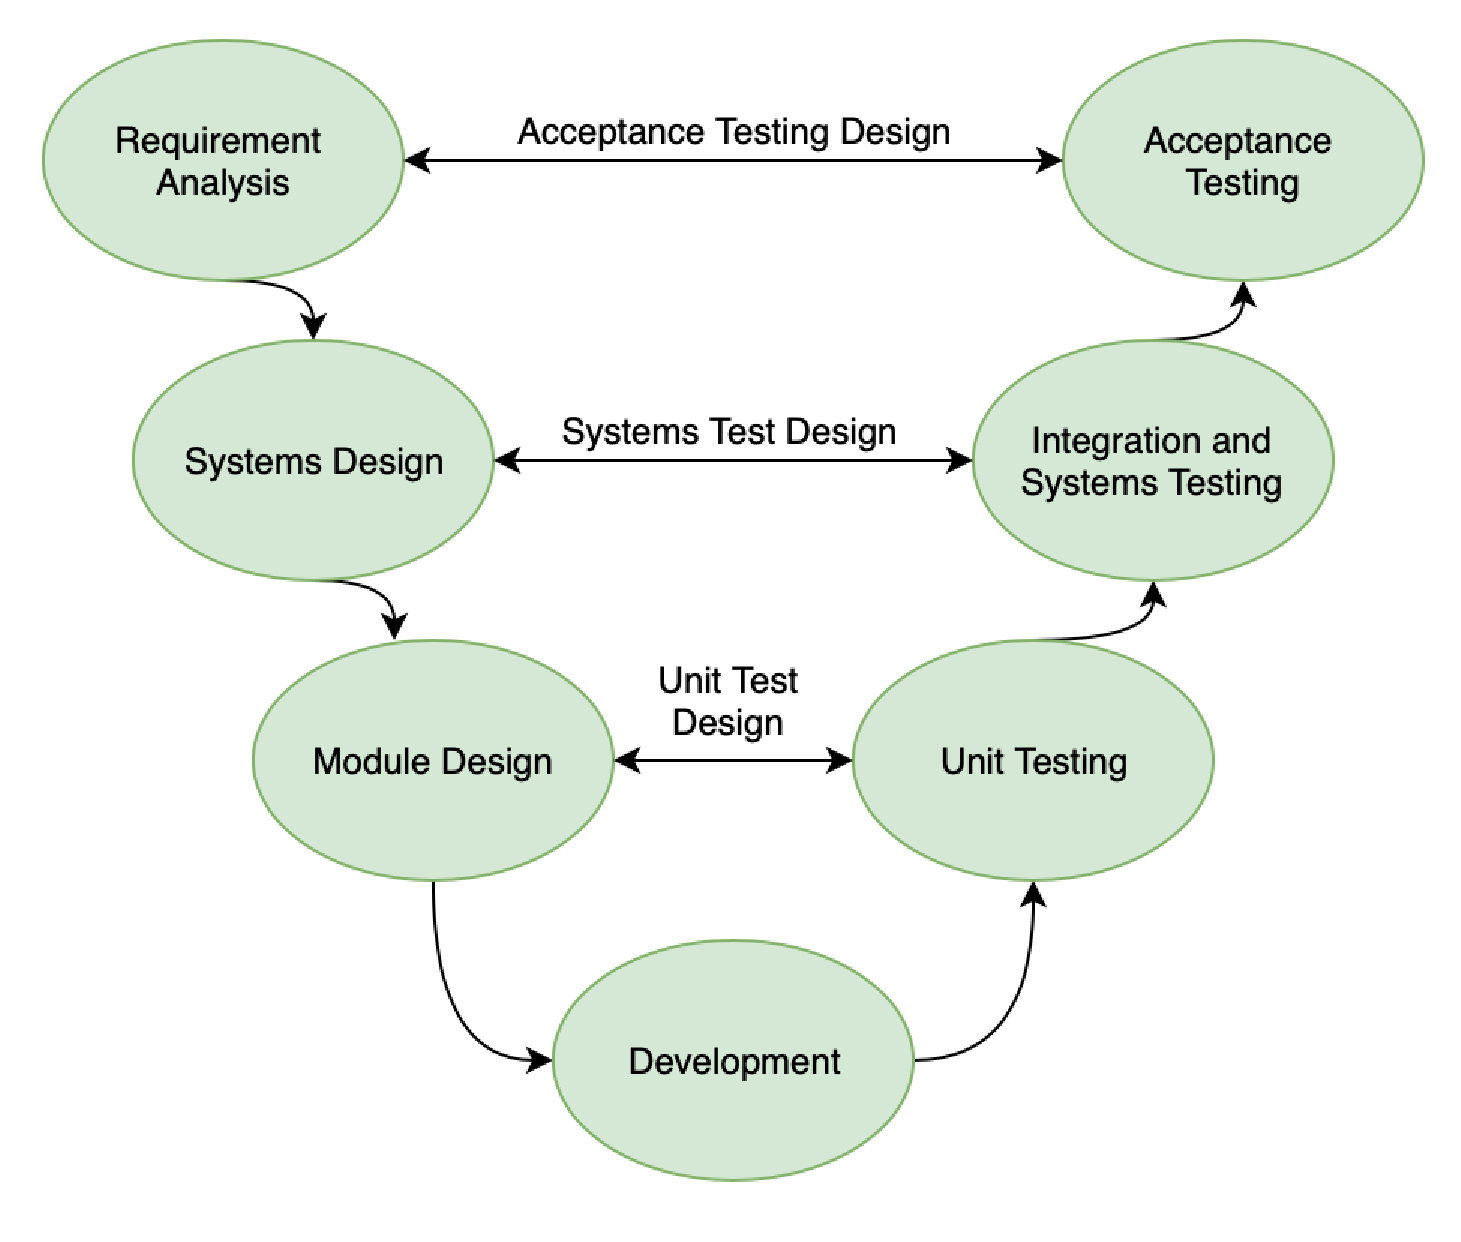
\includegraphics[width = 0.5\textwidth]{images/V-Model.pdf}
    \caption{V-Model used for Design, Implementation and Testing \cite{noauthor_software_2018}} \label{V-Model}
\end{figure}

\section{Systems Design of the Radar}
The system needs to consist of the basic components set out in Figure \ref{pic:overview}. In the following sections, all of the individual subsystems would be tested and an appropriate component would be chosen for the final radar. Figure \ref{pic:overview} displays the basic layout of the system and different variations of this system would be experimented with.

\begin{figure}[h!]
    \centering
    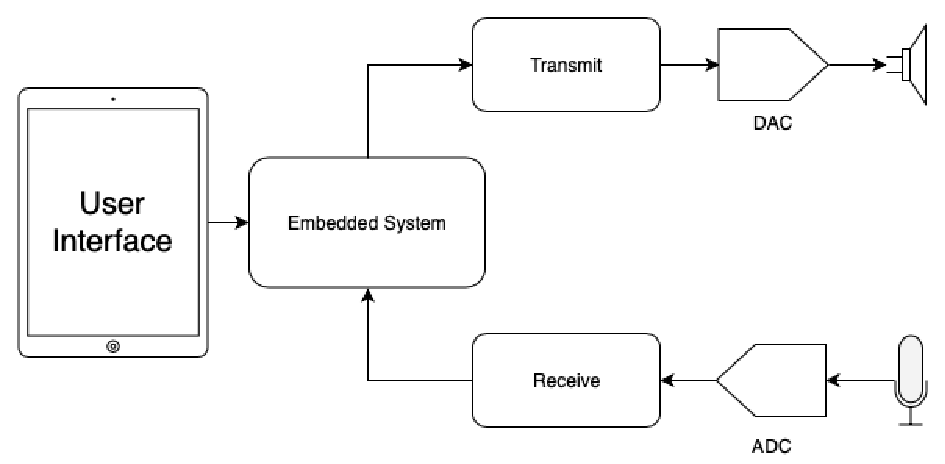
\includegraphics[width = 0.7\textwidth]{images/overview.pdf}
    \caption{Overview of Technical Requirements}\label{pic:overview}
\end{figure}

\section{Module Design}
\subsection{Embedded Platform}
The transmission and receiving sections of the radar can be accommodated on the Teensy 3.6 microcontroller. The Teensy board has a 32 bit 180 MHz ARM Cortex-M4 processor with the ability to process FFT's in real-time. The Teensy with an Audio Shield sold separately, offers $I^2S$ audio output and input. The Teensy 3.6 can be seen in Figure \ref{fig:teensy36} and the Audio Shield in Figure \ref{fig:teensyaudio}. 

\begin{figure}[h!]
    \centering
    \begin{minipage}{0.45\textwidth}
        \centering
        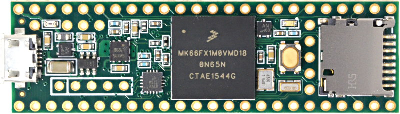
\includegraphics[width=0.9\textwidth]{images/teensy36.pdf}
        \caption{Teensy 3.6}\label{fig:teensy36}
    \end{minipage}\hfill
    \begin{minipage}{0.45\textwidth}
        \centering
        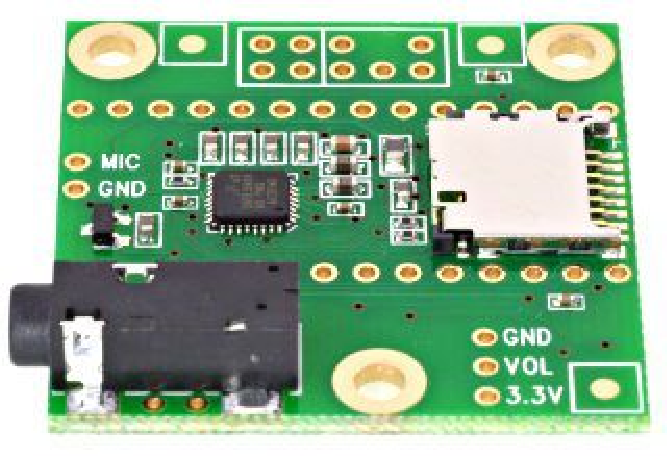
\includegraphics[width=0.9\textwidth]{images/teensy3_audio.pdf}
        \caption{Audio Shield for Teensy 3}\label{fig:teensyaudio}
    \end{minipage}
\end{figure}

The audio is of CD-quality being sampled at $44.1\ KHz$ and $16$-bits and streams automatically as the Arduino script executes. The Teensy board was benchmarked against other Teensy and Arduino boards where it came out on top. The results can be seen in Figure \ref{pic:teensyfft}\cite{chip_open_2016}.

\begin{figure}[h!]
    \centering
    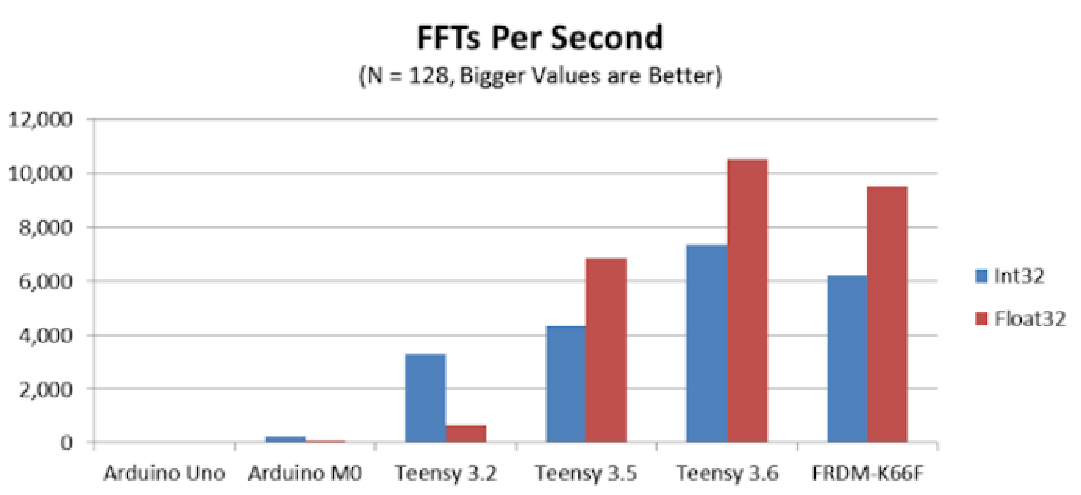
\includegraphics[width = 0.6\textwidth]{images/teensyfft.pdf}
    \caption{Overview Teensy performance in FFT}\label{pic:teensyfft}
\end{figure}

The Teensy board could be used to interface to a speaker using the on-board digital-to-analogue converter (DAC) to play the audio and also to use the on-board ADC to record the returning sound using a microphone. The board can perform FFTs in real-time which is needed to process the received signal. However, the Teensy only has $256\ kb$ of on-board random access memory (RAM) and hosting a user interface without the need for an external PC would be difficult.

The second option is to use the Raspberry Pi 3B (RPi) as an embedded platform. The RPi is a credit card-sized mini-computer with Quad Core 1.2GHz Broadcom BCM2837 64bit central processing unit (CPU) and $1GB$ of RAM. The RPi is not inherently a real-time operating system (RTOS) like Arduino or Teensy boards. Yet it offers faster processor speeds and more RAM for signal processing and a user interface. The RPi does not have an onboard DAC or ADC. Figure \ref{fig:rpi3b} shows the Raspberry Pi 3B.

\begin{figure}[h!]
    \centering
    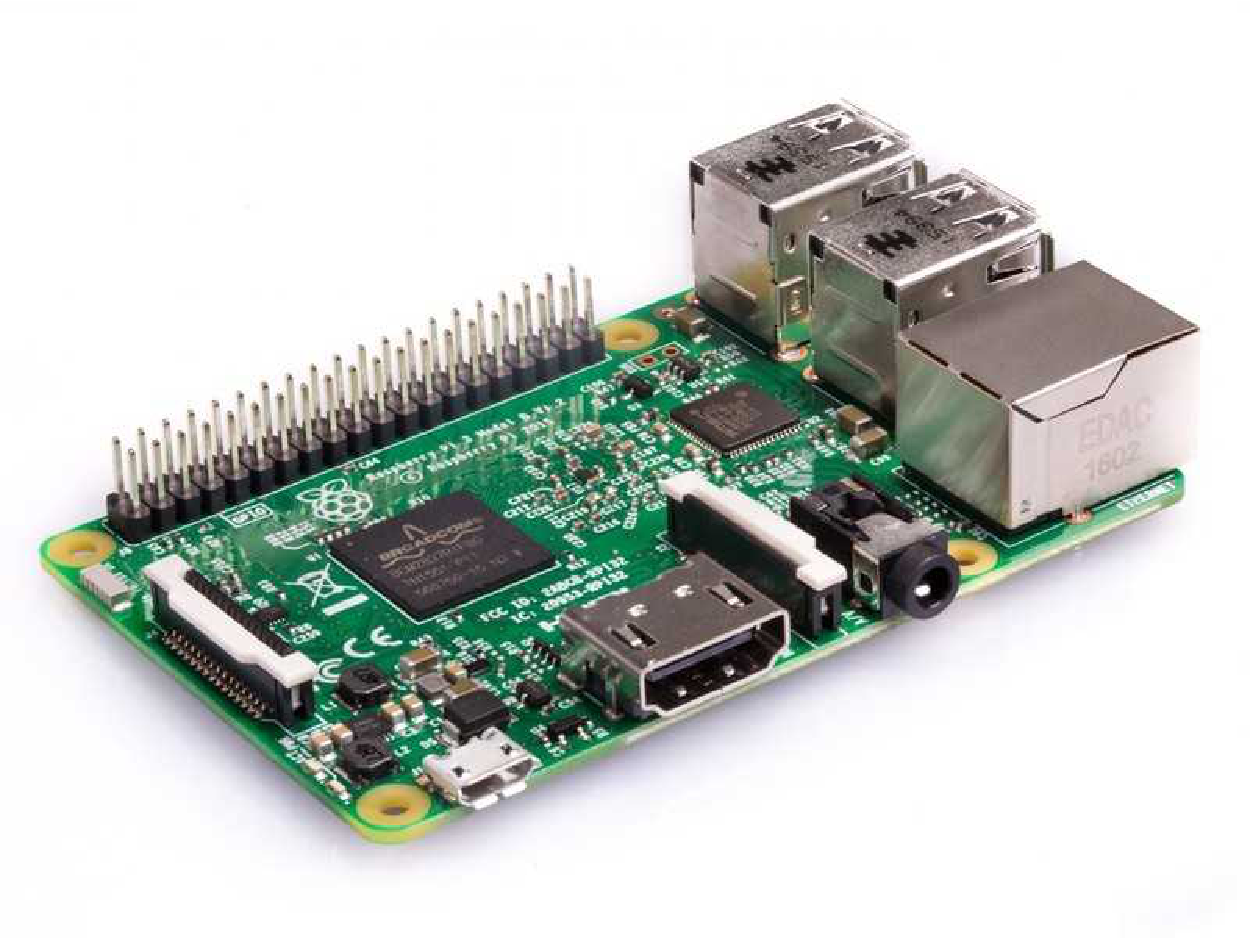
\includegraphics[width = 0.5\textwidth]{images/rpi3b.pdf}
    \caption{Raspberry Pi 3B}\label{fig:rpi3b}
\end{figure}

The two platform's key components and performance are compared head to head in Table \ref{table:comparisonRPiTeensy}.

\begin{table}[h!]
\centering
\begin{tabular}{lll}
\hline
 & \textbf{Teensy 3.6 \cite{noauthor_teensy_nodate}} & \textbf{Raspberry Pi 3B \cite{noauthor_buy_nodate}} \\ \hline
\textbf{Processor} & \begin{tabular}[c]{@{}l@{}}\\ 180 MHz ARM \\ Cortex-M4\end{tabular} & \begin{tabular}[c]{@{}l@{}}1.2 GHZ quad-core \\ ARM Cortex A53\end{tabular} \\
\\ \textbf{RAM} & 256 KB & 1 GB SDRAM \\
\textbf{\begin{tabular}[c]{@{}l@{}}Communication\\ Protocols\end{tabular}} & \begin{tabular}[c]{@{}l@{}}\\USB, Serial, SPI, \\ I2C, CAN Bus\end{tabular} & \begin{tabular}[c]{@{}l@{}}I2C, SPI, UART, \\ Ethernet, Bluetooth\end{tabular} \\
\textbf{Audio Ability} & \begin{tabular}[c]{@{}l@{}}\\2 ADCs 13 bit\\ 2 DACs 12 bit\end{tabular} & PWM 3.5mm socket \\
\textbf{\begin{tabular}[c]{@{}l@{}}\\ Power\\ Consumption\end{tabular}} & 80 mA\cite{noauthor_what_nodate} & 730 mA\cite{noauthor_power_nodate} \\
\\ \textbf{Price} & \$29.95 & \$35 \\ 
\textbf{Shortcomings} & \begin{tabular}[c]{@{}l@{}}\\ Not enough RAM\\ for webserver.\\ No ability to add\\ monitor.\end{tabular} & \begin{tabular}[c]{@{}l@{}}Only PWM $\sim$11bit \\ audio out.\\ No on-board ADC\end{tabular} \\ \hline
\end{tabular}\caption{Comparison: Raspberry Pi 3B and Teensy 3.6}\label{table:comparisonRPiTeensy}
\end{table}

The boards are both similarly priced. Although the Raspberry Pi does not have on-board audio support, the complexity of the Teensy Audio interfaces is not conducive to an educational device. The readily available breakout boards to add the audio capabilities are also affordable with a large community for support. Furthermore, the Teensy 3.6 board does not have enough RAM and no easy and apparent way to host an interface, the obvious choice is the Raspberry Pi 3B. The RPi offers the ability to host a web server as well as the on-board HDMI port if a monitor is needed to be connected. The superior CPU and RAM on the RPi would aid in doing multiple signal processing algorithms one after another. The result would be displayed to the webserver without much delay. 

\subsection{Transmitting Hardware}
\subsubsection{Speakers}
On the transmitting side of the radar, the speaker needs to have a flat frequency response over the operating range of audible frequencies used by the radar. Three different speakers were tested and their frequency response analysed to obtain the speaker with the flattest response.

Firstly, the Visaton Oval Speaker offered a different shape to the usual round speakers. This leads to a wider beam of sound in the narrower axis speaker dimension. Since the radar would be used in louder environments like open-days, it is worth experimenting with. Secondly, the RS Pro unflanged speaker offers the same nominal power to as the Visaton Oval Speaker but has a waterproof PET dome. The speaker doesn't need to be waterproof but it is yet an affordable option. Finally, the RS Pro flanged speaker with a nominal power of $1\ W$ was chosen for the convenience of mounting the speaker and to test whether a less powerful speaker would be sufficient. Table \ref{table:speakers} shows the specifications of each speaker.

\begin{table}[h!]
\centering
\begin{tabular}{lllll}
\hline
\textbf{} & \textbf{Impedence} & \textbf{\begin{tabular}[c]{@{}l@{}}Nominal\\ Power\end{tabular}} & \textbf{Price} & \textbf{Shape} \\ \hline
\textbf{\begin{tabular}[c]{@{}l@{}}\\ Visaton\\ (Flanged)\end{tabular}} & $8 \Omega$ & $2 W$ & R 140.74 & Oval \\
\textbf{\begin{tabular}[c]{@{}l@{}}\\ RS Pro\\ (Unflanged)\end{tabular}} & $8 \Omega$ & $2 W$ & R 59.82 & Round \\
\textbf{\begin{tabular}[c]{@{}l@{}}\\ RS Pro\\ (Flanged)\end{tabular}} & $8 \Omega$ & $1 W$ & R 63.45 & Round \\ \hline
\end{tabular}\caption{Comparison: Speakers}\label{table:speakers}
\end{table}

The frequency response of each speaker was tested in a lab and analysed with a single microphone\footnote{MAX4466 Microphone Pre-Amp Audio Evaluation Board} across all of the speakers. Test conditions were as follow:
\begin{itemize}
\item Signal generator set to $1\ V_{pk-pk}$
\item MAX4466 powered with $5\ V$with bench power supply
\item MAX4466 gain set to $125$x \cite{industries_electret_nodate} 
\item Respective speaker placed on chair $1\ m$ from microphone suspended from the roof \footnote{See Appendix \ref{chap:Testing}}
\item Oscilloscope connected to $OUT$ pin on MAX4466
\item Frequency stepped by $500\ Hz$ starting at $5000\ Hz$ to $15000\ Hz$
\end{itemize}

The results for the speaker frequency response testing for the Visaton speaker can be seen in Figure \ref{fig:Visaton2W}. RS Pro 2W frequency response in Figure \ref{fig:RSPro2W} and the RS Pro 1W in Figure \ref{fig:RSPro1W}.
\begin{figure}[h!]
    \centering
    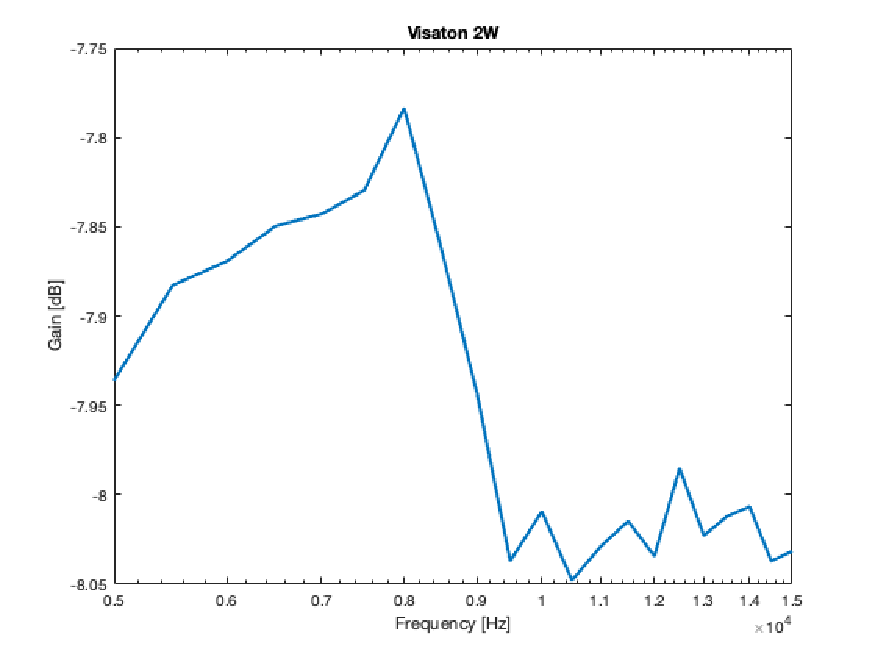
\includegraphics[width = 0.5\textwidth]{images/Visaton2W.pdf}
    \caption{Frequency Response: Visaton 2W}\label{fig:Visaton2W}
\end{figure}
\begin{figure}[h!]
    \centering
    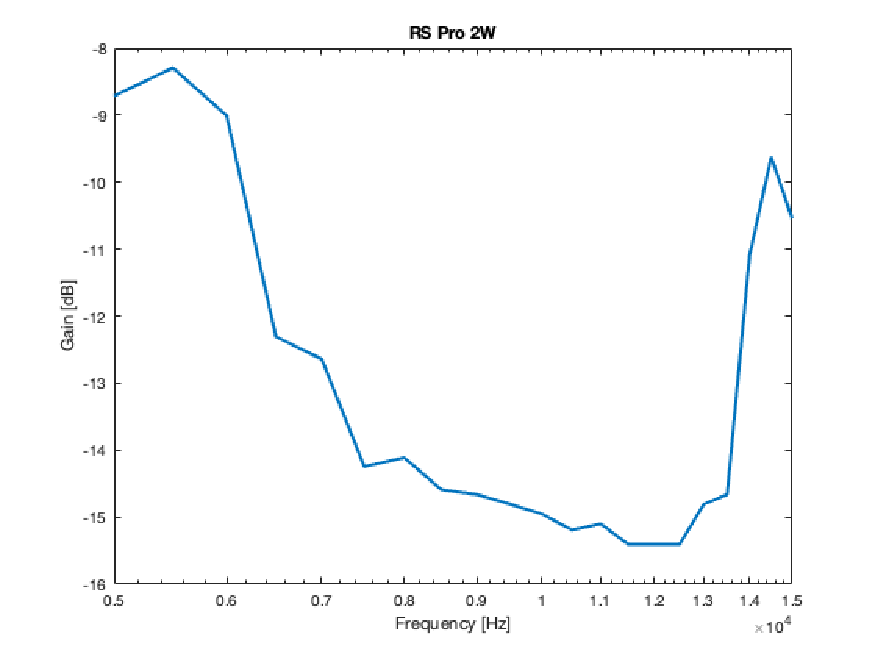
\includegraphics[width = 0.5\textwidth]{images/RSPro2W.pdf}
    \caption{Frequency Response: RS Pro 2W}\label{fig:RSPro2W}
\end{figure}
\begin{figure}[h!]
    \centering
    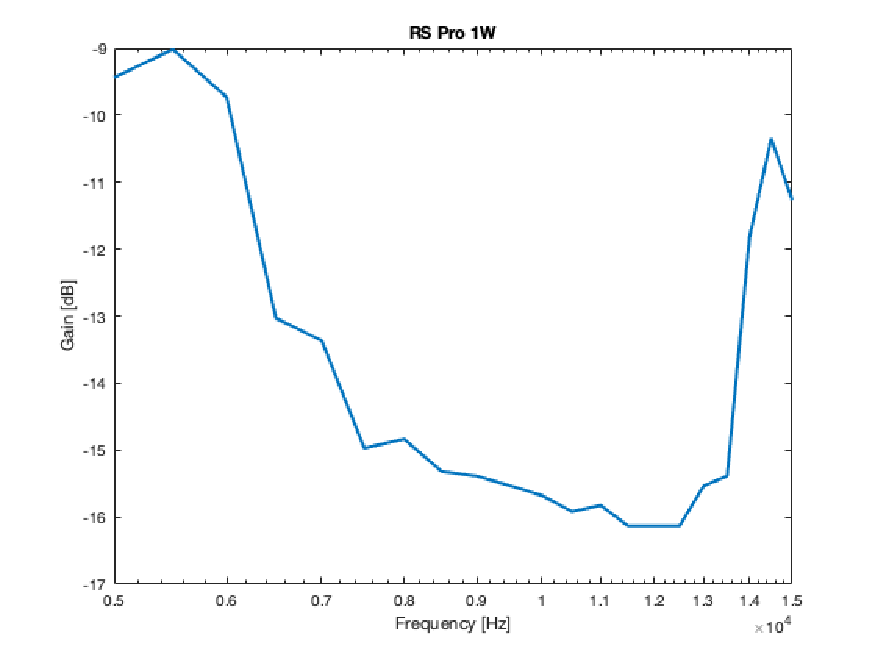
\includegraphics[width = 0.5\textwidth]{images/RSPro1W.pdf}
    \caption{Frequency Response: RS Pro 1W}\label{fig:RSPro1W}
\end{figure}
The frequency responses for the RS Pro speakers are extremely similar because they follow a similar design except for the nominal power rating that differs (therefore the higher gain associated with it) and the 2W speaker does not have a flange for mounting. Both the RS Pro speakers show a relatively flat response over the intended operating frequency of $8000\ Hz$ to $12000\ Hz$. The Visaton speaker shows an erratic response over the operating frequency having a sharp decline at $8000\ -\ 9500\ Hz$.

The RS Pro $1\ W$ proved to be more than sufficient for the operating frequencies and the flanged design makes for easy mounting in a finished product. The speaker is not the most powerful but the response is comparable to that of the $2\ W$ speakers.

\subsubsection{Digital-to-Analogue Converter (DAC)}

Following the speaker tests, the DAC needed to be investigated to see that we have a linear and accurate response from the devices. The  DACs need to take in a digital signal and convert it to an analogue signal for playing over a speaker. The DAC investigated is the Adafruit MAX98357 $I^2S$ Class-D Mono Amp that features a $I^2 S$ digital audio device specifically made for microcontrollers. If the microcontroller has the ability of $I^2 S$ digital audio, like the Raspberry Pi and Teensy both support, the breakout board takes in digital audio, converts it to analogue, and amplifies it. When the device is powered with $5\ V$, the output is a maximum of $3.2\ W$on $4 \Omega$ impedance and 10\% total harmonic distortion (THD) or $1.8\ W$ on $8 \Omega$ with 10\% THD \cite{noauthor_adafruit_nodate}. 

The amplifier used is the device which would introduce non-linearities to the system. The frequency response of the device could not be tested individually since it is part of a complete breakout board. The datasheet, however, does support the hypothesis that the response is roughly linear in the operating range. Figure \ref{fig:ampfreq} shows the normalised frequency response of the MAX98357A amplifier when supplied with $5\ V$ and the gain set to $12\ dB$.
\begin{figure}[h!]
    \centering
    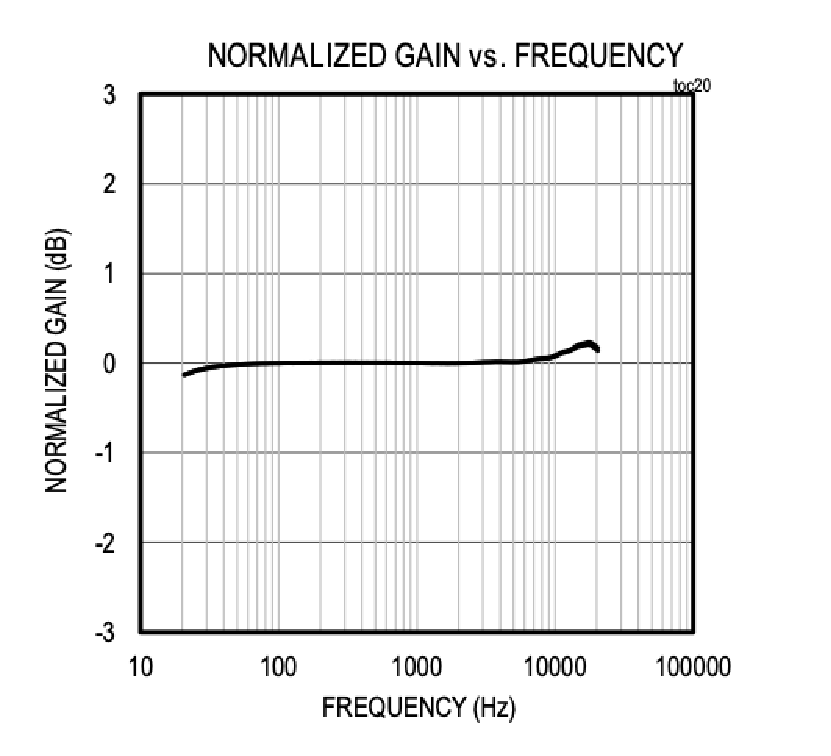
\includegraphics[width = 0.5\textwidth]{images/ampfreq.pdf}
    \caption{Frequency Response: MAX98357A Amplifier \cite{noauthor_max98357a_2019}}\label{fig:ampfreq}
\end{figure}

\subsection{Receiving Hardware}
\subsubsection{Microphone}
The receiving side of the radar, the microphone forms a vital part and its operation is crucial to the workings of a radar. Therefore, the frequency response is important since the signal processing would require accurate frequency pick up by the microphone. A similar approach to testing the speakers was followed to test the microphones. 

Two different microphones were tested where the first is a breakout board with an adjustable gain set with a screwdriver on the back called the MAX4466 also used for testing frequency response of the speakers. The second microphone is the MAX9814 breakout board with an automatic gain. This ensures that the output from the microphone never clips the signal. Both of these microphones can be supplied with $2.4\ V -\ 5.5\ V$making them both suitable for use with the RPi or the Teensy 3.6. 

To ensure consistency in the testing of the microphones, a single speaker\footnote{MacBook Pro 2015 right-hand speaker} was used at a distance of $1\ m$. The Set up can be seen in Appendix \ref{chap:Testing}. The $OUT$ pins from both microphones were connected to an oscilloscope to measure their frequency response between $5000\ Hz\ -\ 15000\ Hz$ in steps of $500\ Hz$. Figure \ref{fig:MAX4466} shows the frequency response of the MAX4466 with its gain set to a maximum. Figure \ref{fig:MAX9814} shows the frequency response of the MAX9814 with automatic gain. 

\begin{figure}[h!]
    \centering
    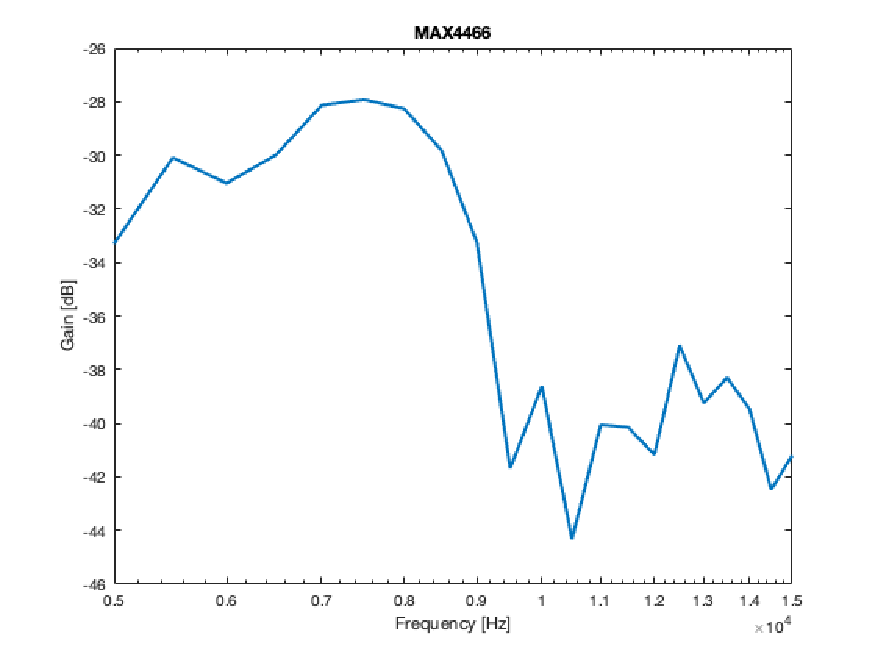
\includegraphics[width = 0.5\textwidth]{images/MAX4466.pdf}
    \caption{Frequency Response: MAX4466 Microphone} \label{fig:MAX4466}
\end{figure}

\begin{figure}[h!]
    \centering
    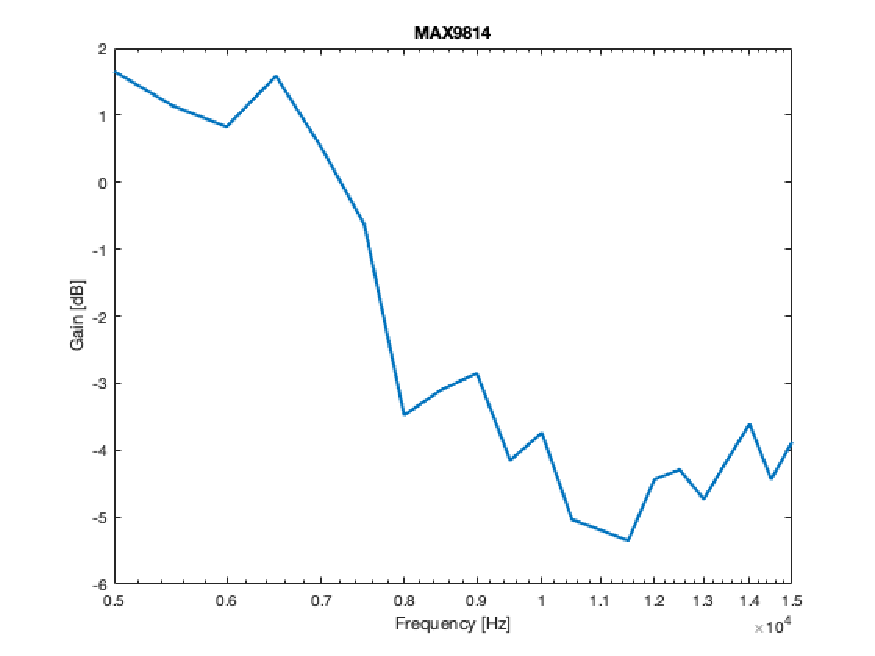
\includegraphics[width = 0.5\textwidth]{images/MAX9814.pdf}
    \caption{Frequency Response: MAX9814 Microphone}\label{fig:MAX9814}
\end{figure}

Both of the microphones have a relatively flat frequency response over the radar's operating frequency. However, there are some inconsistencies in both microphones especially with the MAX4466 at higher frequencies. It should also be noted that the MAX4466 output voltage is significantly lower than that of the MAX9814 since the automatic gain of the microphone amplifies the quieter signal from the computer a lot more efficiently compared to the single setting gain. Therefore, MAX9814 microphone would be prefered to the adjustable gain microphone to work better in noisy environments where the radar might be used. All of the recorded data sets to verify the testing of the microphones and speakers can be found along with all the screenshots and photos taken, \href{https://github.com/DewanPieterse/AudioRadar/tree/master/Matlab}{\underline{here}}. 


\subsubsection{Analogue-to-Digital Converter (ADC)}
To convert the analogue signal obtained by the microphone, an ADC is required for the microcontroller to be able to process the data as a digital signal. The Nyquist sampling rate \cite{landau_sampling_1967}, which states that a signal must be sampled at or above at least twice the highest frequency that needs to be observed, need to be satisfied. To sample in the audible frequency range with a maximum of $20\ 000\ Hz$, the sampling rate should be at least $40\ 000\ Hz$. Ideally, the sampling rate of $44\ 100\ Hz$ is desirable since this frequency is CD quality and sound frequencies are identifiable. Three options were considered for this process. 

The first ADC is the MCP3008 I/P which offers a sampling rate of $200$ kilo samples per second (ksps) when powered by a $5\ V$ supply. The device offers a $10$ bit resolution over 8 channels. The device is compact and widely used with microcontrollers and the low cost of the device makes it a competitive choice. A sampling resolution of $10$ bits are not necessarily desirable but given the uncertainty regarding sampling rates and equally timed samples, this remains an option. Figure \ref{fig:mcp3008} shows the physically small size of the device.

\begin{figure}[h!]
    \centering
    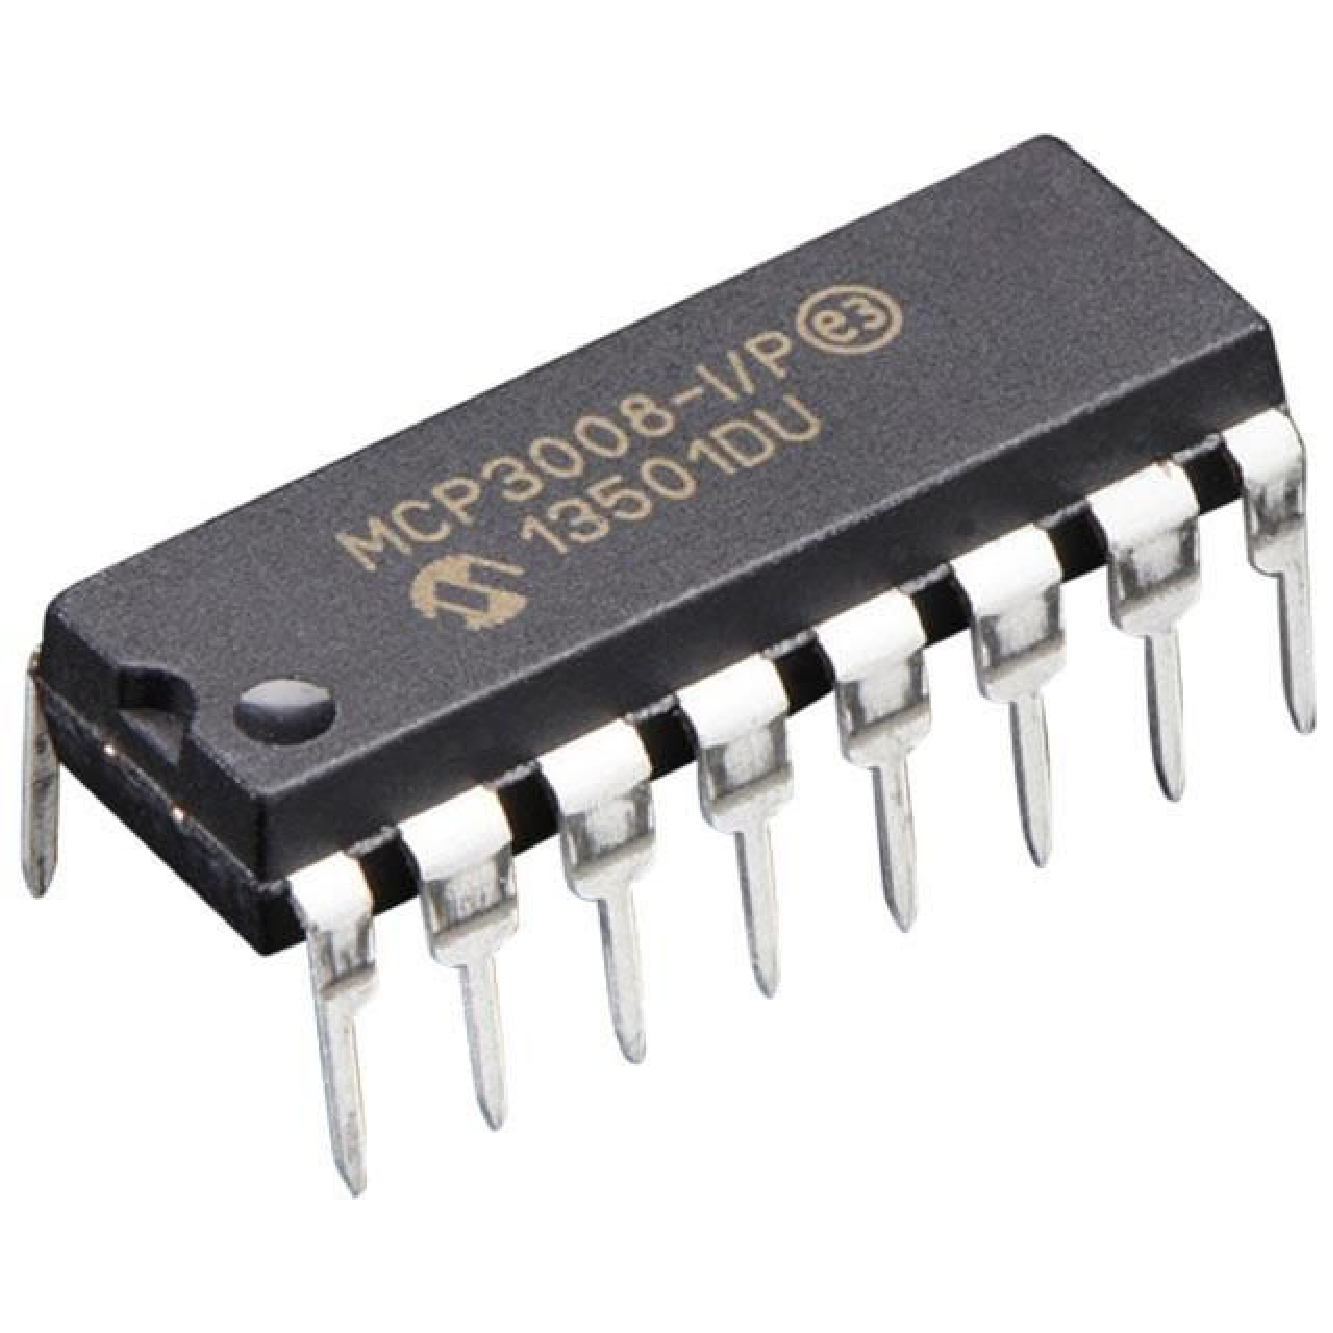
\includegraphics[width = 0.3\textwidth]{images/mcp3008.pdf}
    \caption{MCP3008-I/P physical package \cite{noauthor_mcp3008_nodate}}\label{fig:mcp3008}
\end{figure}

Initial tests using the Raspberry Pi and the SPI interface that the MCP3008 uses only offered a sampling rate of about $8000\ Hz$. This was as a result of each sample with the MCP3008 took 24 clock cycles to read the value. Therefore, this option delivered insufficient results.

Secondly, the Teensy 3.6 microcontroller was considered having a $16$ bit ADC on-board. It can communicate with a Raspberry Pi through the USB port using UART. The Teensy board is flashed using the Teensyduino plugin and programmed using the standard Arduino IDE in C. This lends itself to be an easily programmable board with vast amounts of support online through forums and communities. The Teensy was used in conjunction with the RPi and sound recorded using the MAX9814 microphone. The code for the Teensy can be found in Appendix \ref{Appendix:Code}. Initial results with the Teensy proved that the recorded sound reflected the tone that was generated using MATLAB. The code is also available in Appendix \ref{Appendix:Code}. Figure \ref{fig:soundTeensy} shows the tone received and Figure \ref{fig:fftTeensy} shows the FFT of the tone. The tone generated was set to $10\ 000\ Hz$.

\begin{figure}[h!]
    \centering
    \begin{minipage}{0.45\textwidth}
        \centering
        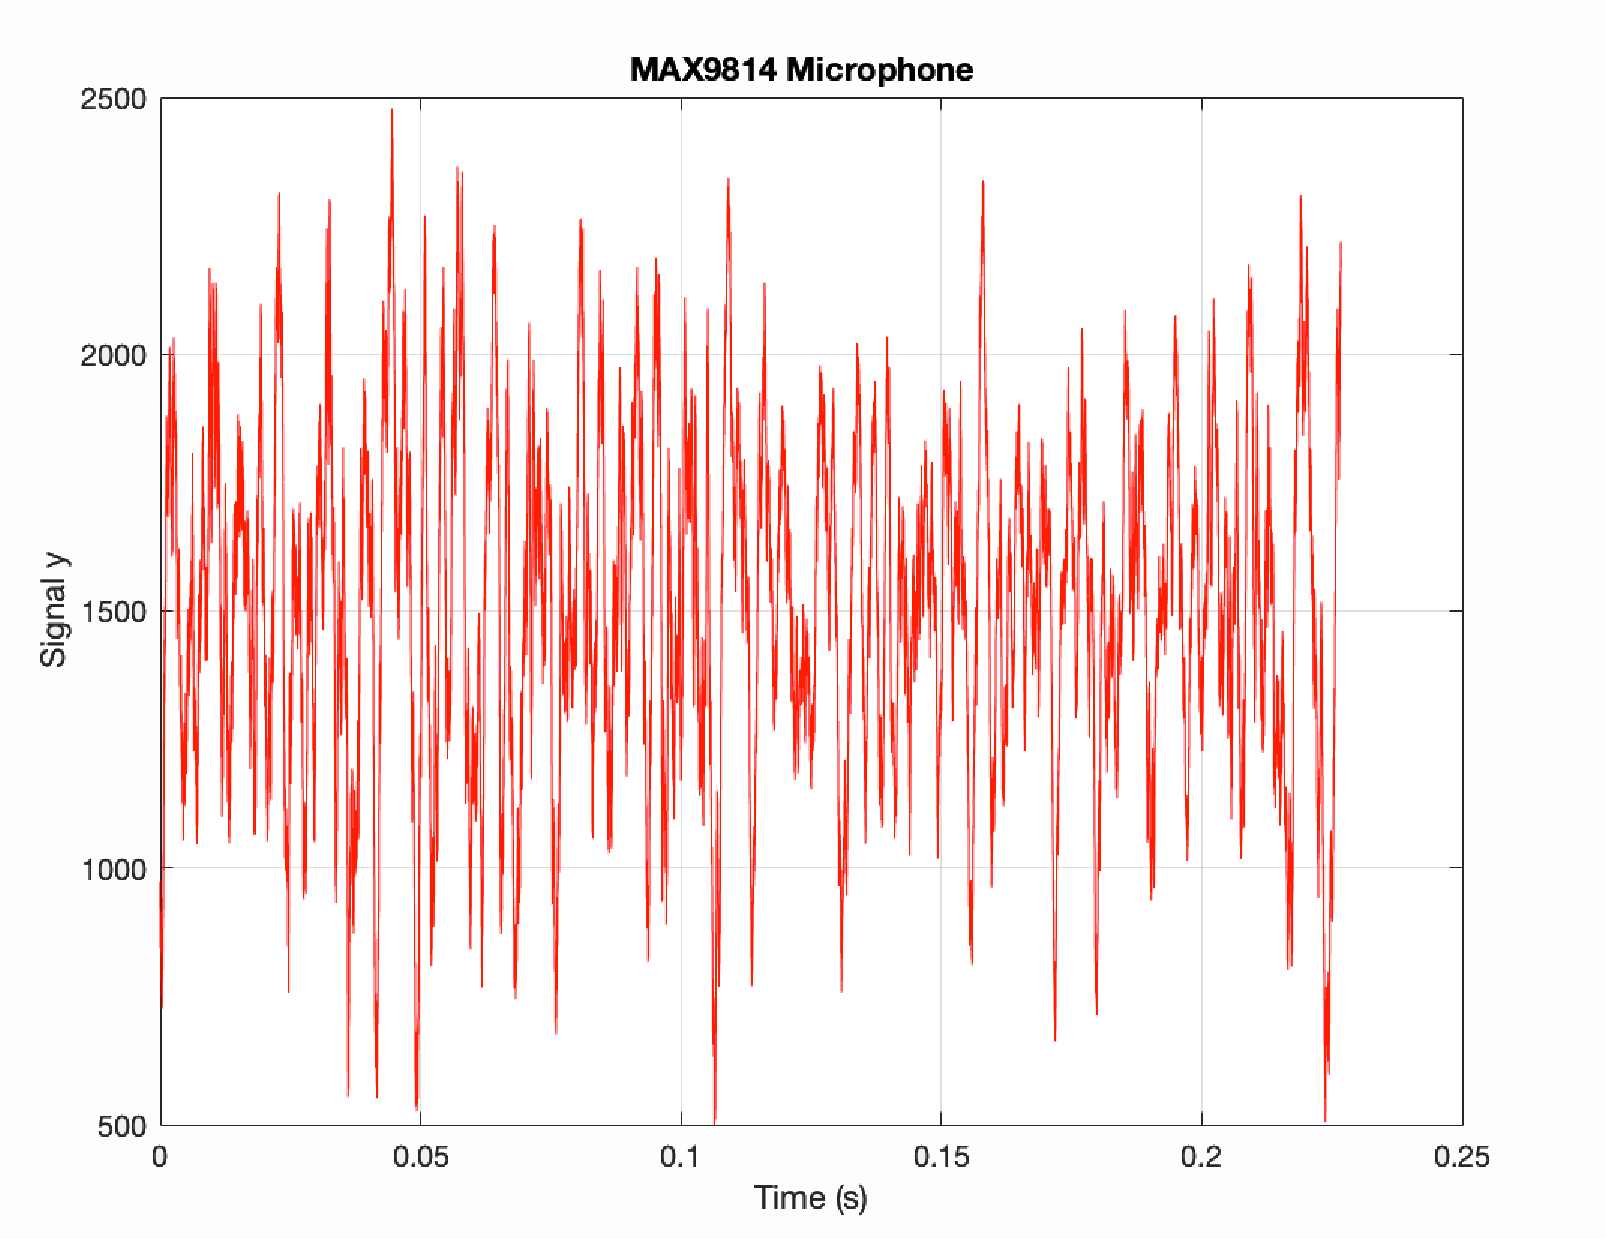
\includegraphics[width=0.9\textwidth]{images/soundTeensy.pdf}
        \caption{$10\ 000\ Hz$ Tone Recorded by Teensy}\label{fig:soundTeensy}
    \end{minipage}\hfill
    \begin{minipage}{0.45\textwidth}
        \centering
        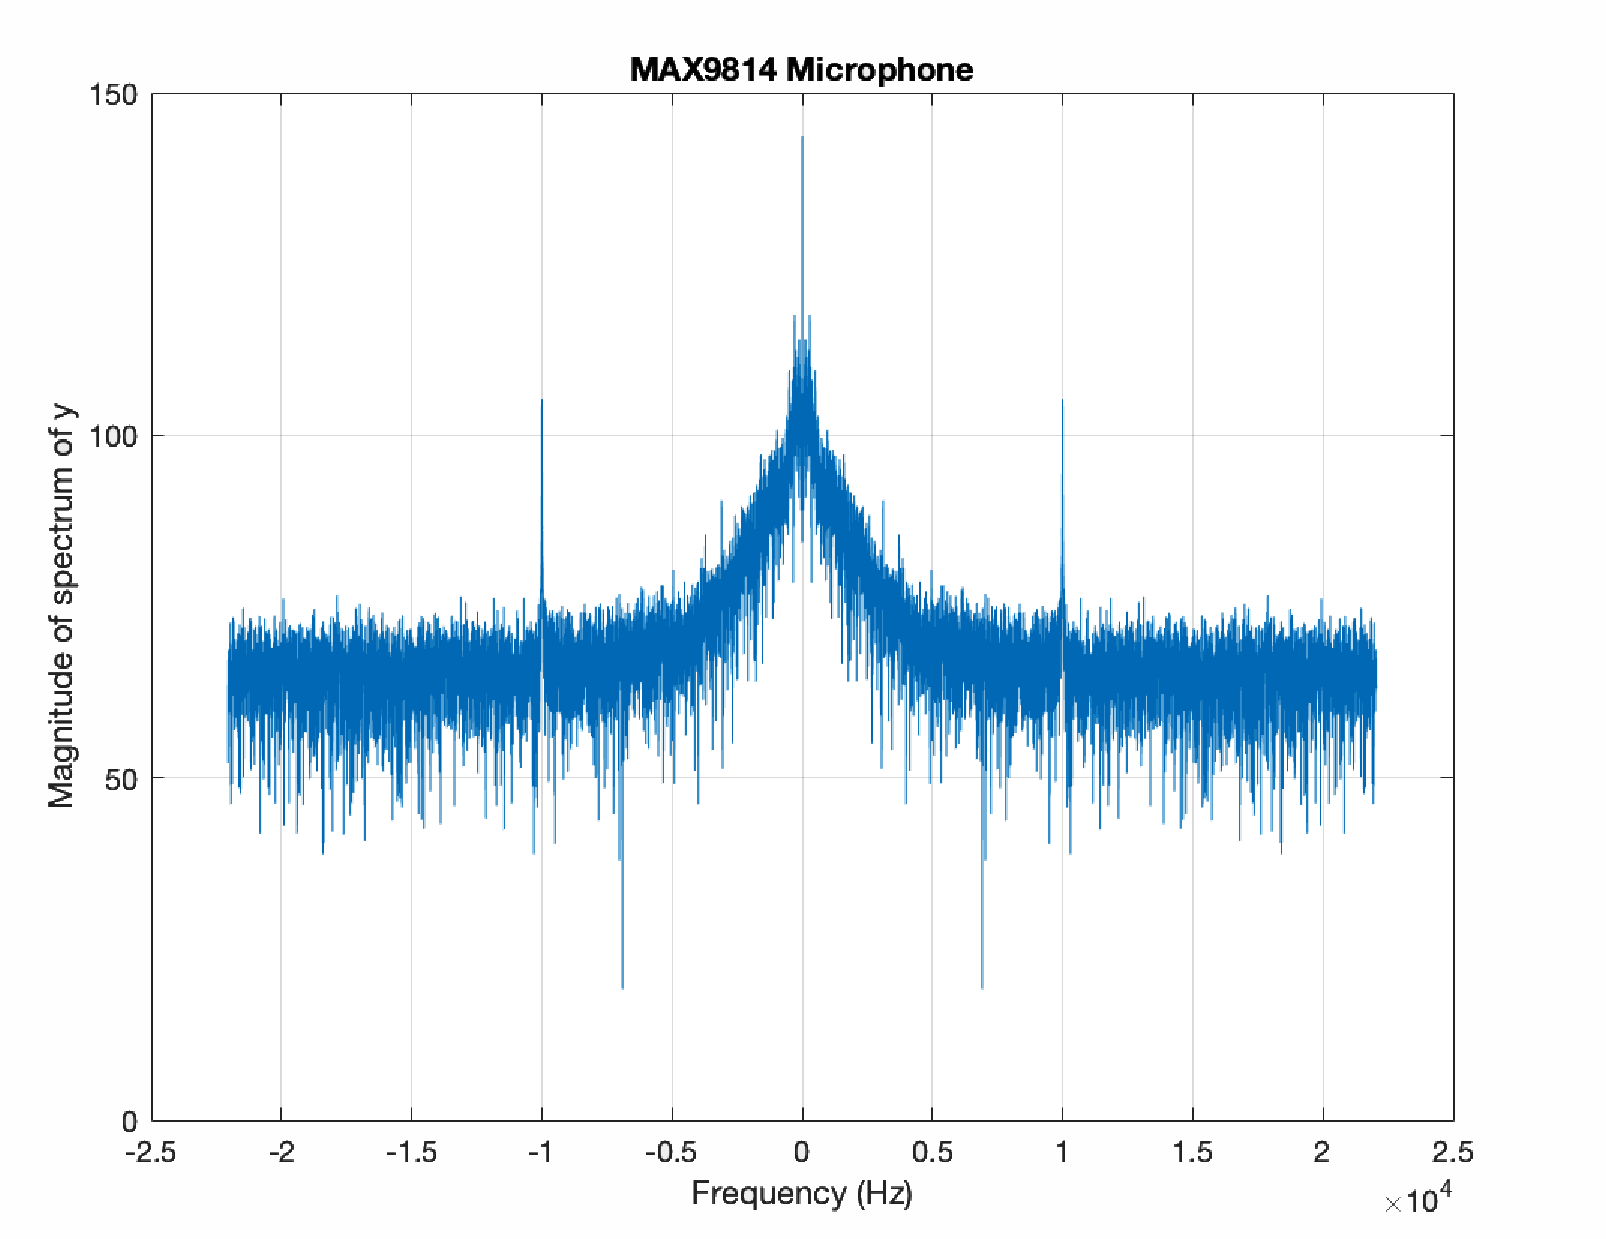
\includegraphics[width=0.9\textwidth]{images/fftTeensy.pdf}
        \caption{FFT of Tone Recorded by Teensy}\label{fig:fftTeensy}
    \end{minipage}
\end{figure}

Figure \ref{fig:fftTeensy} shows that the frequency component is peaking at exactly $10\ 000\ Hz$. However, it is important to note that the maximum duration to stream in real-time, using the PySerial package in Python through USB, was only worth $0.224\ s$ of sound data. This renders the Teensy, is only used as an ADC, expensive and not sufficient for recording tones long enough for processing in a radar.

Finally, a USB sound card compatible with Raspberry Pi was tested. The Astrum 3D Sound Card features a mono microphone input socket for audio recording. It also has an audio out but the radar requires that the microphone record and the speaker play at the same time and this device does not allow for simultaneous recording and playing. The sound card samples audio through the input jack at $44\ 100\ Hz$ at $16$ bit sample resolution. This is a sufficient sampling rate and CD quality. Therefore, suitable for the radar. Figure \ref{fig:9000} shows a visual representation of a spectrum of frequencies ($9\ 000\ Hz$ in this case over $1\ s$) called a spectrogram and shows how accurately the sound was recorded.

\begin{figure}[h!]
    \centering
    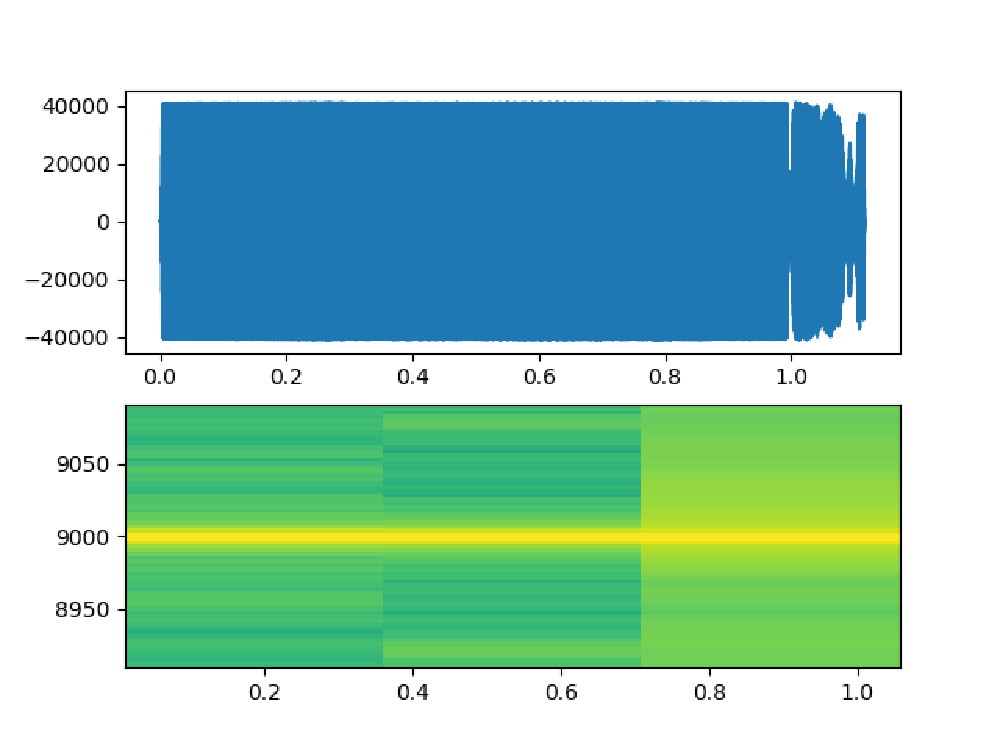
\includegraphics[width = 0.5\textwidth]{images/9000.pdf}
    \caption{Received tone and spectrogram of $9\ 000\ Hz$ tone}\label{fig:9000}
\end{figure}

The spectrogram at $9\ 000\ Hz$ shows that the ADC sound card samples the data at a sufficient rate with a resolution exceeding the requirements. Table \ref{table:adcComp} shows the direct comparison between the most important parameters of the three options considered.

\begin{table}[h!]
\begin{tabular}{lllll}
\hline
\centering
\textbf{} & \textbf{\begin{tabular}[c]{@{}l@{}}Practical\\ Sampling Rate\end{tabular}} & \textbf{\begin{tabular}[c]{@{}l@{}}Sampling \\ Resolution\end{tabular}} & \textbf{Price} & \textbf{\begin{tabular}[c]{@{}l@{}}Ease of\\ implementation\end{tabular}} \\ \hline
\\ \textbf{MCP3008} & $8\ ksps$ & $10\ bit$ & R 27.11 & Decent \\
\\ \textbf{Teensy 3.6} & $44.1\ ksps$ & $16\ bit$ & \$ 29.95 & Hard \\
\\ \textbf{\begin{tabular}[c]{@{}l@{}}Astrum USB\\ Sound Card\end{tabular}} & $44.1\ ksps$ & $16\ bit$ & R 99 & Easy \\ \hline
\end{tabular}\caption{Comparison: ADC parameters}\label{table:adcComp}
\end{table}

Therefore, it can be concluded that the USB sound card, given the low-cost, CD-quality sampling ability, and the ease of use, is the ADC of choice for the radar project.

\subsection{Software}
The software used to host a web app needs to have the ability to be easily understandable as well as easy to implement given the requirements of the project. Two options that were investigated were Flask and Django, and both have proved to be widely popular under python web developers.

\subsubsection{Django}

Django is considered a full-stack web development platform. It offers developers the ability to implement common web site protocols without much effort. It does, however, lack some common features that Python offer. Django is considered to be an environment with all the add-ons and functionality already included in its source, leaving nothing out to develop a fully operational web application. It offers everything from an admin panel to database structures right out of the box.

It is considered to be a 'batteries included' approach to web application development \cite{dwyer_flask_nodate}.


\subsubsection{Flask}
Flask offers the minimum tools to get a web application working and if additional functionality is sought after, the flask framework is open to third-party applications and packages. It is more simplistic in its design and it lets you decide how, and whether you want a certain functionality implemented. 

Flask is considered to be a more explicit implementation of Python and that makes it easier to read the code and understand what is happening \cite{dwyer_flask_nodate}.

\subsubsection{Software Comparison}
Table \ref{table:software101} shows the direct comparison between Flask and Django.

\begin{table}[h!]
\centering
\begin{tabular}{lll}
\hline
\textbf{} & \textbf{Django} & \textbf{Flask} \\ \hline
\\\textbf{\begin{tabular}[c]{@{}l@{}}Resource \\ Intensive\end{tabular}} & Medium footprint & Light footprint \\
\\\textbf{Simplicity} & \begin{tabular}[c]{@{}l@{}}Harder to read,\\ implement\end{tabular} & \begin{tabular}[c]{@{}l@{}}Easily readable and \\ implemented\end{tabular} \\
\\\textbf{\begin{tabular}[c]{@{}l@{}}Built-in\\ Functionality\end{tabular}} & All-inclusive functionality & \begin{tabular}[c]{@{}l@{}}Not a lot of functionality\\ out-of-the-box\end{tabular} \\
\\\textbf{Expandability} & Medium & High \\
\\\textbf{Support} & \begin{tabular}[c]{@{}l@{}}2631 StackOverflow\\ questions \cite{dwyer_flask_nodate}\end{tabular} & \begin{tabular}[c]{@{}l@{}}575 StackOverflow\\ questions \cite{dwyer_flask_nodate}\end{tabular} \\ \hline
\end{tabular}\caption{Software Comparison}\label{table:software101}
\end{table}

Therefore, for the simplicity and the functional working of Flask, it was chosen as the preferred software package to use to implement the web app. As stated in \cite{dwyer_flask_nodate}, Flask is also more focused on the experience and educational aspect of development. The Raspberry Pi is also not the most powerful computer and hence the lightweight footprint of the software contributes to the choice.

\subsubsection{Software Implementation and Testing}

A Flask web application was set up to run on the Raspberry Pi. An HTML template was generated using Bootstrap Studio to improve on the user experience. The packages imported into Python include:

\begin{itemize}
\item \verb request  used to process forms submitted to the app.
\item \verb render_template  used to render the HTML templates for the user interface.
\item \verb Flask  is used to implement and initiate the Flask web application.
\end{itemize}

Seven web pages were developed to aid in both a technical and non-technical implementation of the Continuous Wave and the Pulsed-Doppler radar modes. One of the pages is for a home (landing) page, one for an error handling and the other a results page. Each web page is scalable to fit the width of 4 different devices\footnote{Widescreen desktop, desktop, tablet and phone}. Figure \ref{fig:website1} shows the web application implemented on a tablet-sized screen.

\begin{figure}[h!]
    \centering
    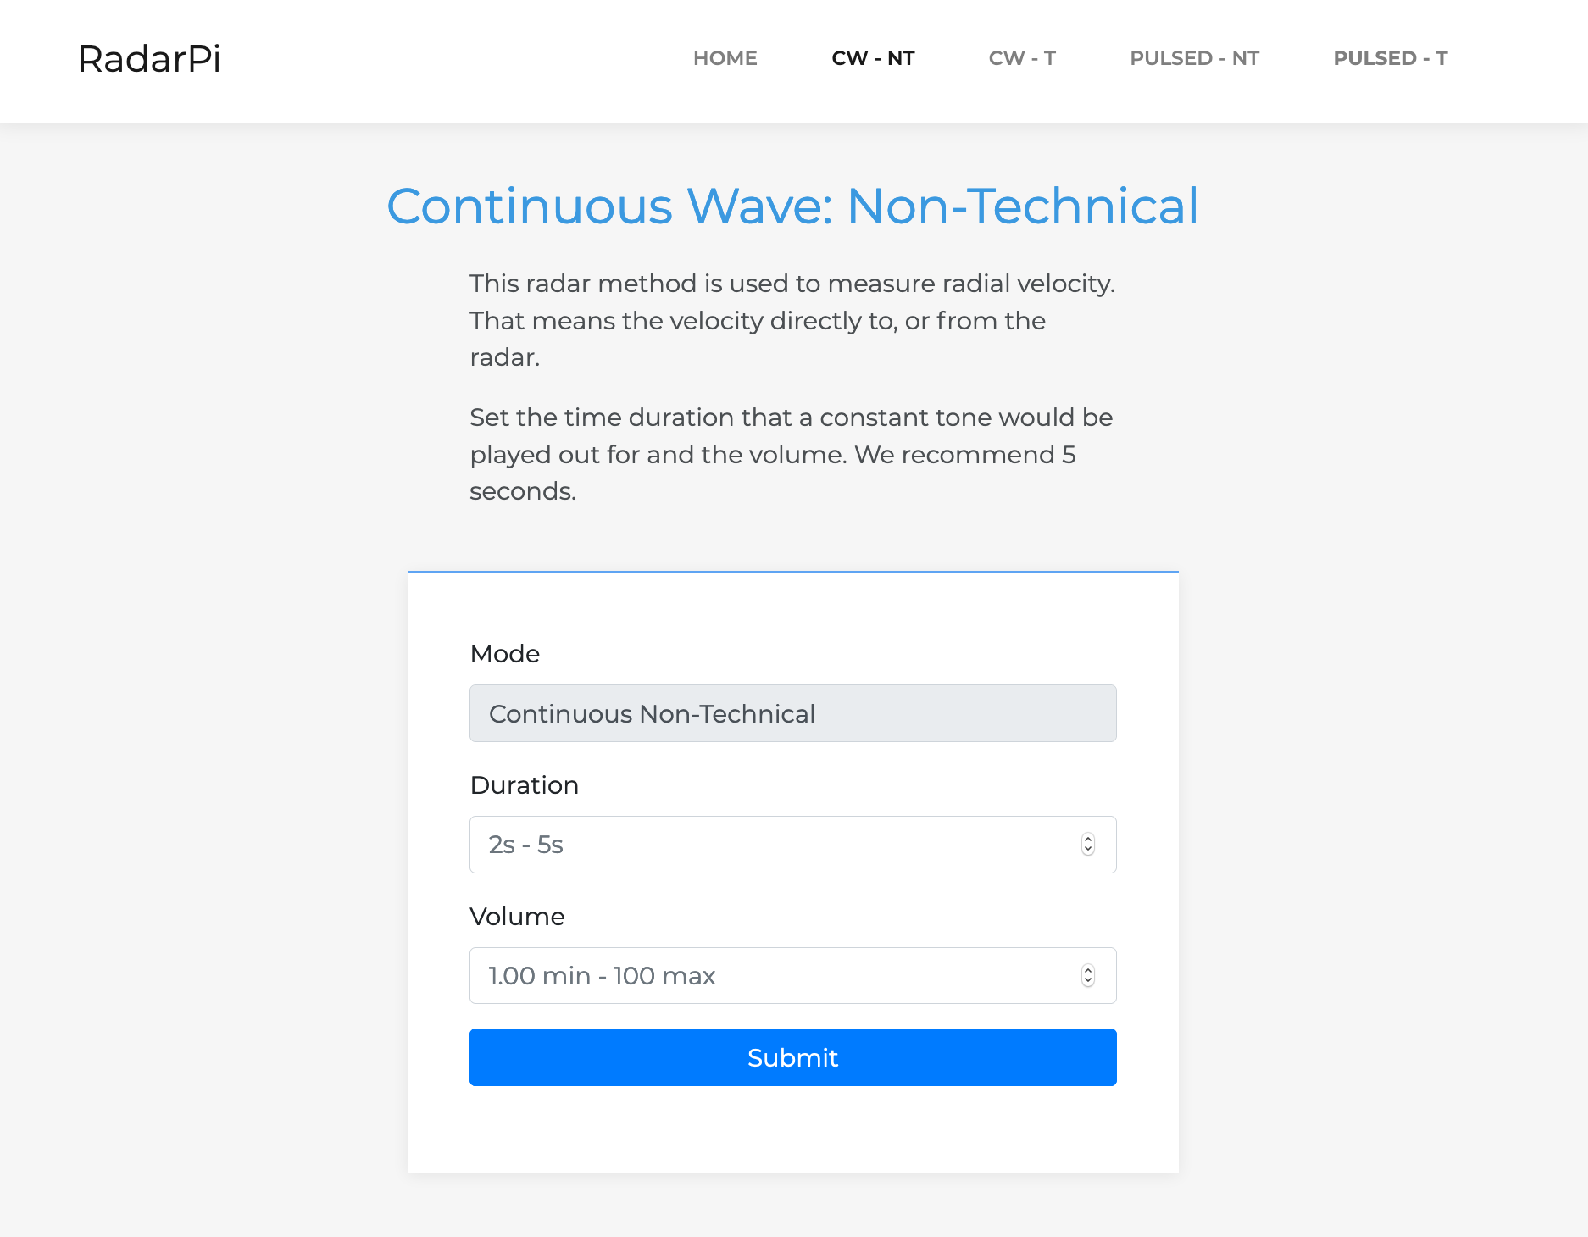
\includegraphics[width = 0.8\textwidth]{images/website1.pdf}
    \caption{Website User Interface: Continuous Wave (Non-Technical)}\label{fig:website1}
\end{figure}

Figure \ref{fig:website2} shows the web application displaying results after testing the continuous wave radar by rapidly approaching and retreating a hand to and from the radar.

\begin{figure}[h!]
    \centering
    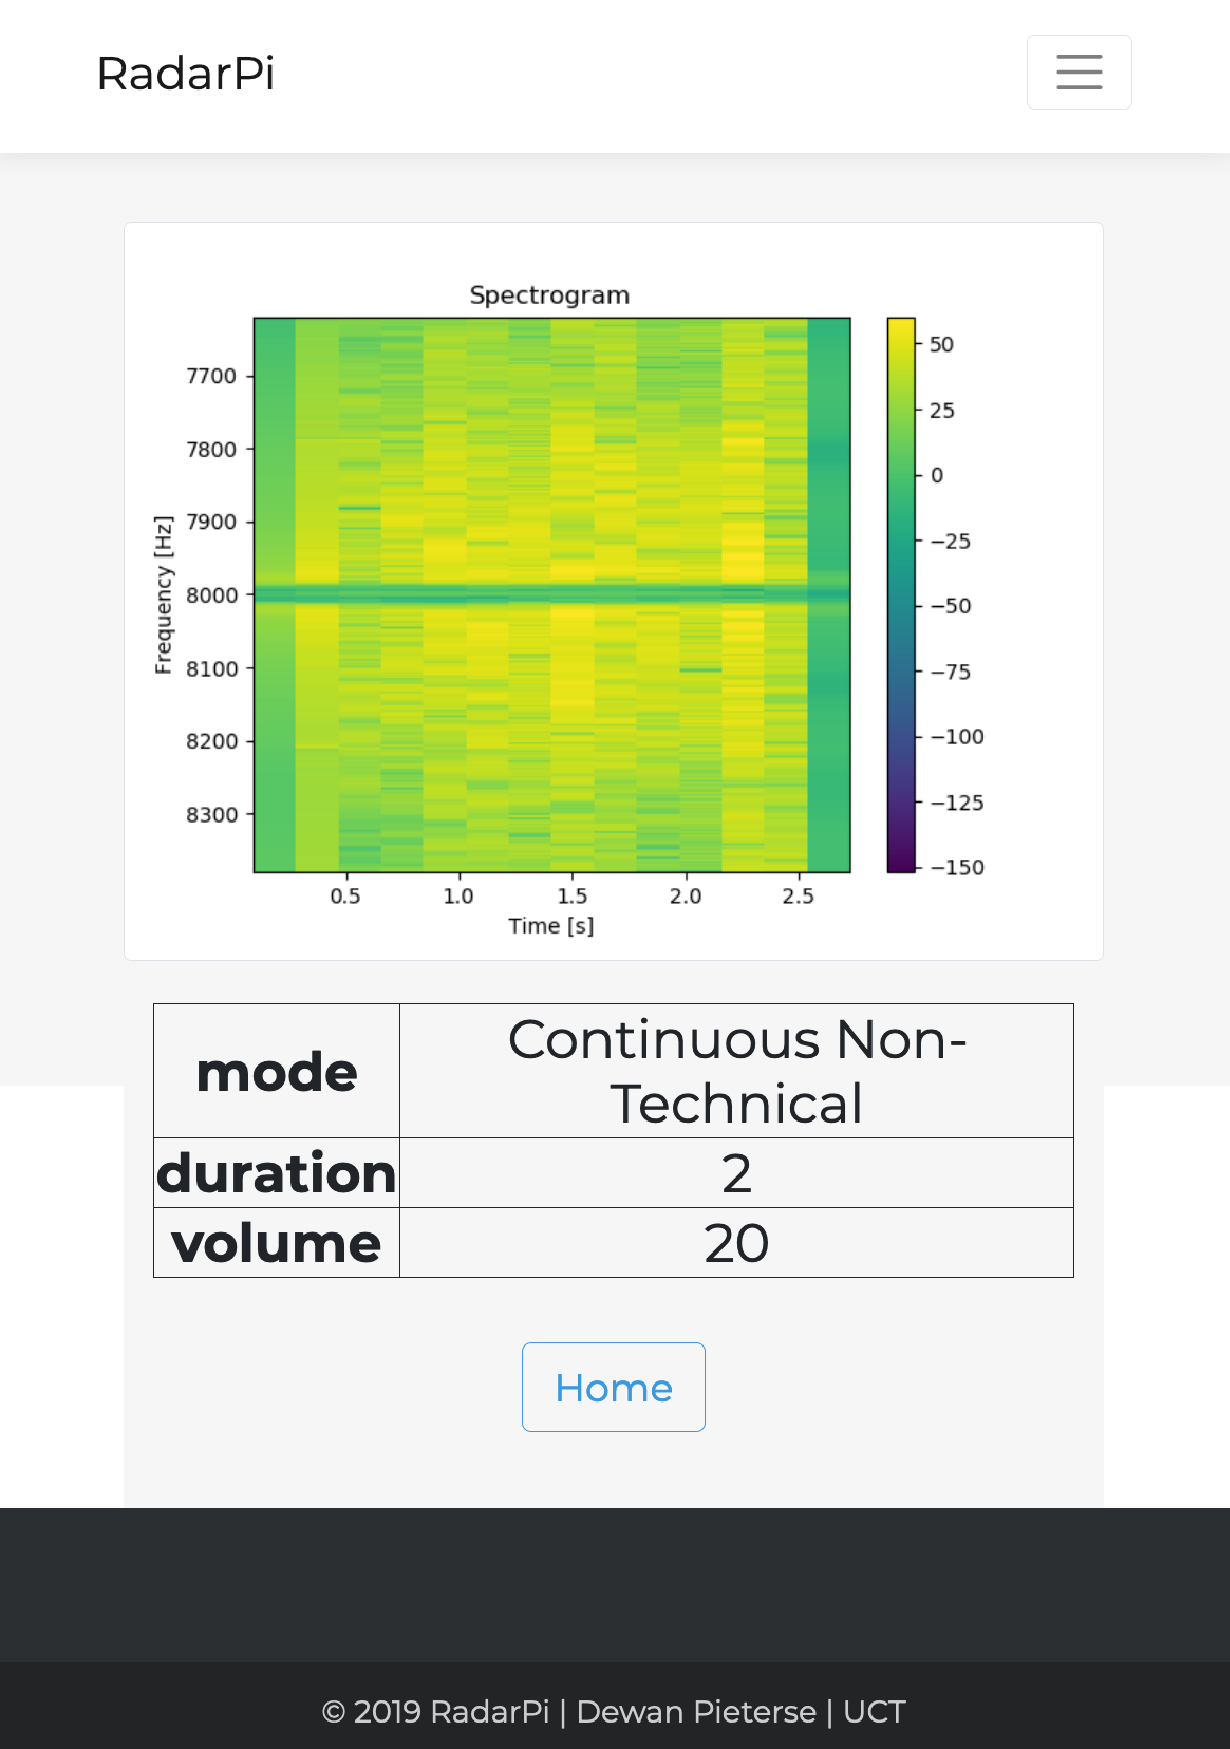
\includegraphics[width = 0.6\textwidth]{images/website2.pdf}
    \caption{Website User Interface: Results}\label{fig:website2}
\end{figure}

\subsection{Enclosure Design\label{enclosureDesign}}
A simple enclosure was sought after to merely protect the components and render the radar to be portable. Figure \ref{fig:lidOn} shows the basic design for the enclosure from the front with the lid on while Figure \ref{fig:lidOff} shows the components visible with the lid removed.

\begin{figure}[h!]
    \centering
    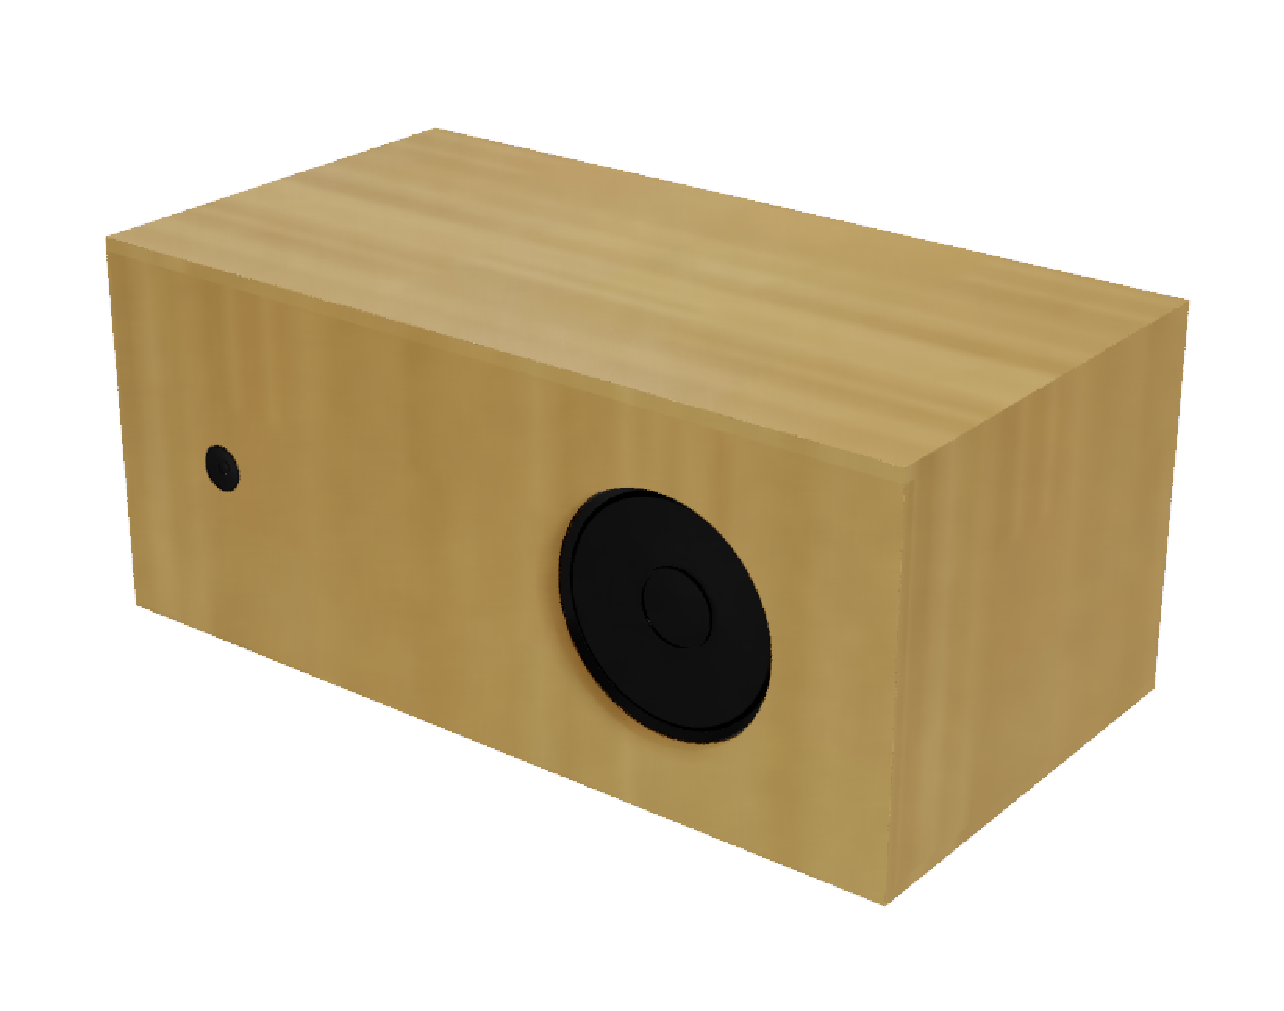
\includegraphics[width = 0.5\textwidth]{images/lidOn.pdf}
    \caption{Enclosure with Lid Installed}\label{fig:lidOn}
\end{figure}

\begin{figure}[h!]
    \centering
    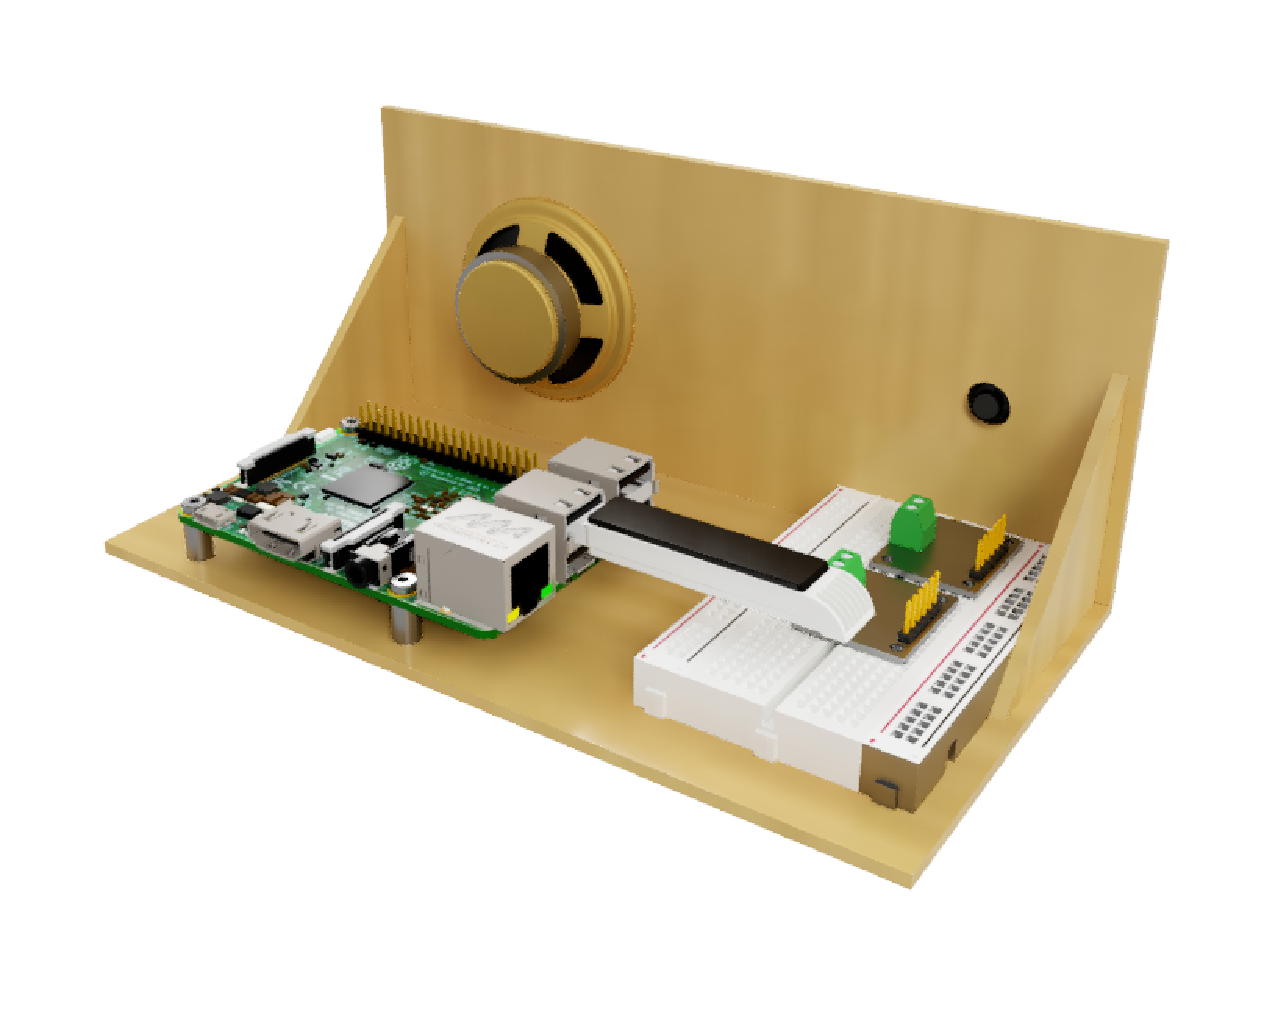
\includegraphics[width = 0.5\textwidth]{images/lidOff.pdf}
    \caption{Enclosure with Components Visible}\label{fig:lidOff}
\end{figure}

\section{Selection Summary}
Table \ref{table:compSelect} shows the summary of all the selected subsystems after being tested and scrutinised. The budget constraint is also satisfied in the table.

\begin{table}[h!]
\centering
\begin{tabular}{lll}
\hline
\textbf{Component} & \textbf{Selection} & \textbf{Price} \\ \hline
\textbf{\begin{tabular}[c]{@{}l@{}}\\ Embedded \\ Platform\end{tabular}} & Raspberry Pi 3B & R 534.25 \\ \\
\textbf{Speaker} & \begin{tabular}[c]{@{}l@{}}RS Pro $1\ W$\\ (Flanged)\end{tabular} & R 63.45 \\ \\
\textbf{DAC} & \begin{tabular}[c]{@{}l@{}}Adafruit MAX98357 $I^2S$ \\ Class-D Mono Amp\end{tabular} & R 85 \\ \\
\textbf{Microphone} & Adafruit MAX9814 & R 228.25 \\ \\
\textbf{ADC} & Astrum USB Sound Card & R 99 \\ \\ 
\textbf{\begin{tabular}[c]{@{}l@{}}Web App \\ Software\end{tabular}} & Flask & Open-source \\  \hline
 &  & R1009.95 \\ \cline{3-3} 
\end{tabular}\caption{Final component selection}\label{table:compSelect}
\end{table}

It is important to note that the remaining budget would be partly spent on the enclosure, although only a small amount. The low cost is a user requirement of the radar as specified in Section \ref{UserReqs}.

\newpage
\section{Signal Processing of the Radar}
The signal processing of the radar is the process where the signals are created to be played out and the analysis and processing of the received signal as received by the microphone. The processes followed will use the received data to ultimately generate a Range-Doppler Map where the radial distance to an object will be visible as highlighted colours and the velocity of an object in the case of the Continuous Wave Radar.

The Range-Doppler map would be obtained with generating a set number of pulses consisting of chirps where the velocity map would be obtained with a constant tone using the Doppler Effect (both methods as described in Chapter \ref{chap:Radar Theory}). The following sections show the design of the signal processing used for both applications.

\subsection{Range-Doppler Radar Signal Processing and Implementation}
\subsubsection{Generate Transmit Pulse and Signal}
The transmit pulse and transmit signals are generated using the Numpy Python package and  a cosine function. The time element is generated by the user entering the bandwidth of the chirp where the duration is calculated as:

\begin{equation}
T = \frac{100}{B}
\end{equation}The chirp rate $\mu\ (mu)$, is calculated using the duration and the bandwidth as:
\begin{equation}
\mu = \frac{B}{T}
\end{equation}The single chirp is then generated with the code:
\begin{verbatim}
y = (np.cos(2 * np.pi * (f0 * t + 0.5 * mu * t**2)))
\end{verbatim} 

The individual chirp is then duplicated using the \verb np.tile()  function to generate the pulse train needed for transmission. The transmit pulse of bandwidth $4000\ Hz$, unambiguous range of $10\ m$, the range resolution of $0.05\ m$, and centre frequency of $8000\ Hz$ can be seen in Figure \ref{fig:Tx_p}. The transmit signal can be seen in Figure \ref{fig:Tx_Signal} with $32$
pulses that are just the repeated pulse from the transmitted pulse.

\begin{figure}[h!]
    \centering
    \begin{minipage}{0.45\textwidth}
        \centering
        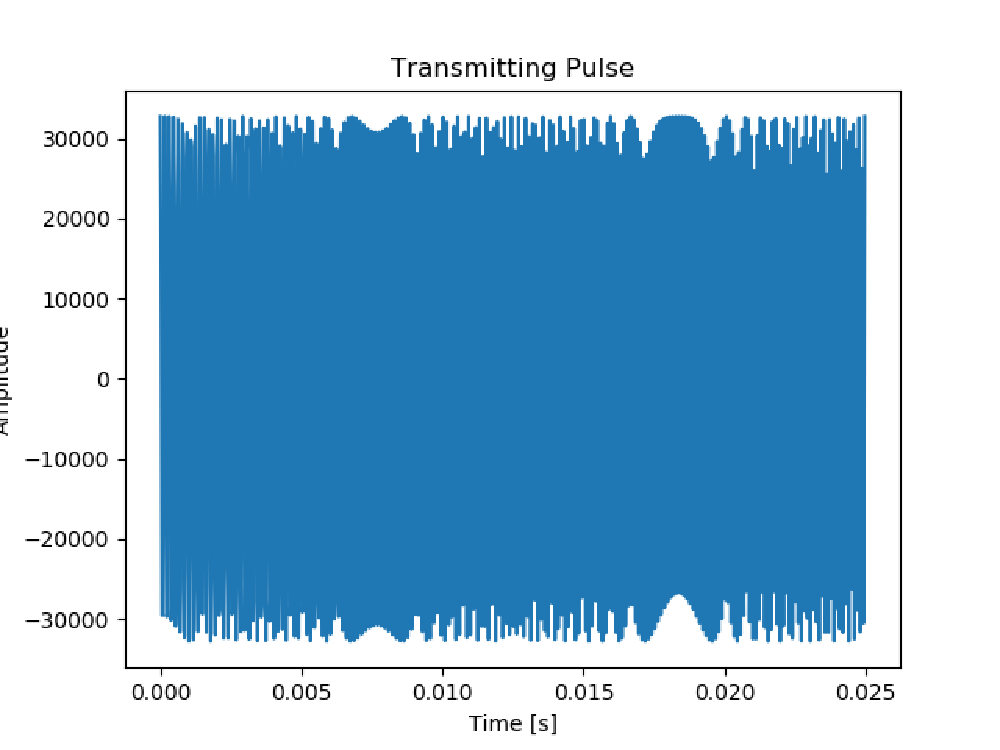
\includegraphics[width=0.9\textwidth]{images/Tx_p.pdf}
        \caption{Transmitting Pulse}\label{fig:Tx_p}
    \end{minipage}\hfill
    \begin{minipage}{0.45\textwidth}
        \centering
        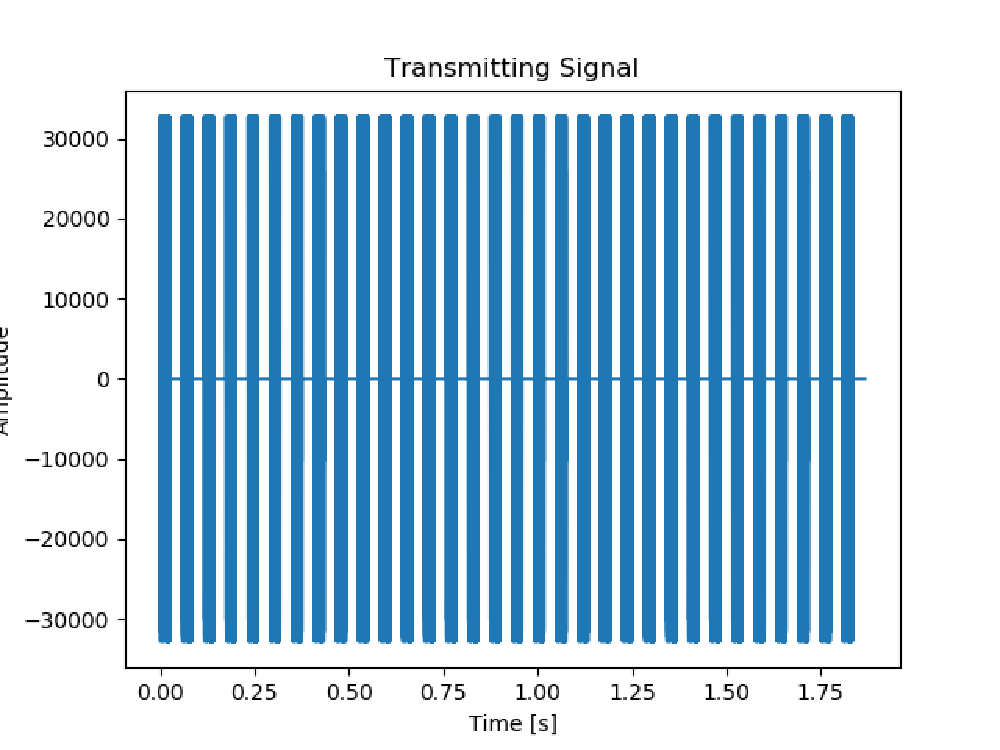
\includegraphics[width=0.9\textwidth]{images/Tx_Signal.pdf}
        \caption{Transmitting Signal}\label{fig:Tx_Signal}
    \end{minipage}
\end{figure}

\subsubsection{Downmixing and Low Pass Filter}
Next, a function was written to implement the downmixing and low pass filtering of the received signal. The function written to implement the downmixing takes in sampling time, the bandwidth of the chirp, centre frequency, the signal itself and the time over which it has been sampled. It returns the downmixed and low pass filtered complex signal in its baseband. The code snippet below shows the function written in Python.

{\small\begin{verbatim}
def downMix(ts,B,fc,signal,time):
    fs = 1/ts
    pi = np.pi
    [numtaps, f] = 101, (fc + B/2)
    coeffsLowPass = scipy.signal.firwin(numtaps, f, pass_zero=False, fs=fs)
    cos = np.cos(2 * pi * fc) * time                                                         # I channel
    I_tp = np.multiply(signal, np.transpose(cos))
    I_tp_LPF = scipy.signal.convolve(I_tp, coeffsLowPass)
    sin = -np.sin(2 * pi * fc ) * time                                                         # Q channel
    Q_tp = np.multiply(signal, np.transpose(sin))
    Q_tp_LPF = scipy.signal.convolve(Q_tp, coeffsLowPass)
    return I_tp_LPF + (1j * Q_tp_LPF)
\end{verbatim}}

\subsubsection{Matched Filter}

The received signal in Figure \ref{fig:rxSignal101} is downmixed and them the matched filter is applied in Python using the code below. The function takes in the complex downmixed received signal and the complex downmixed transmitted pulse and returns the range line that is sought. It has the output that can be seen in Figure \ref{fig:matchedfilterOutput}.

{\small\begin{verbatim}
def matchedFilter(tp,r):
    N1 = len(tp)
    N2 = len(r)
    N3 = N2 - N1; 
    tp_ZP = np.pad(tp, (0, N3), 'constant')
    FFT_conj_tp_ZP = np.conj(fft(tp_ZP))
    FFT_r = fft(r)
    fftTpR = ifft(FFT_conj_tp_ZP * FFT_r)
    return fftTpR
\end{verbatim}}

\begin{figure}[h!]
    \centering
    \begin{minipage}{0.45\textwidth}
        \centering
        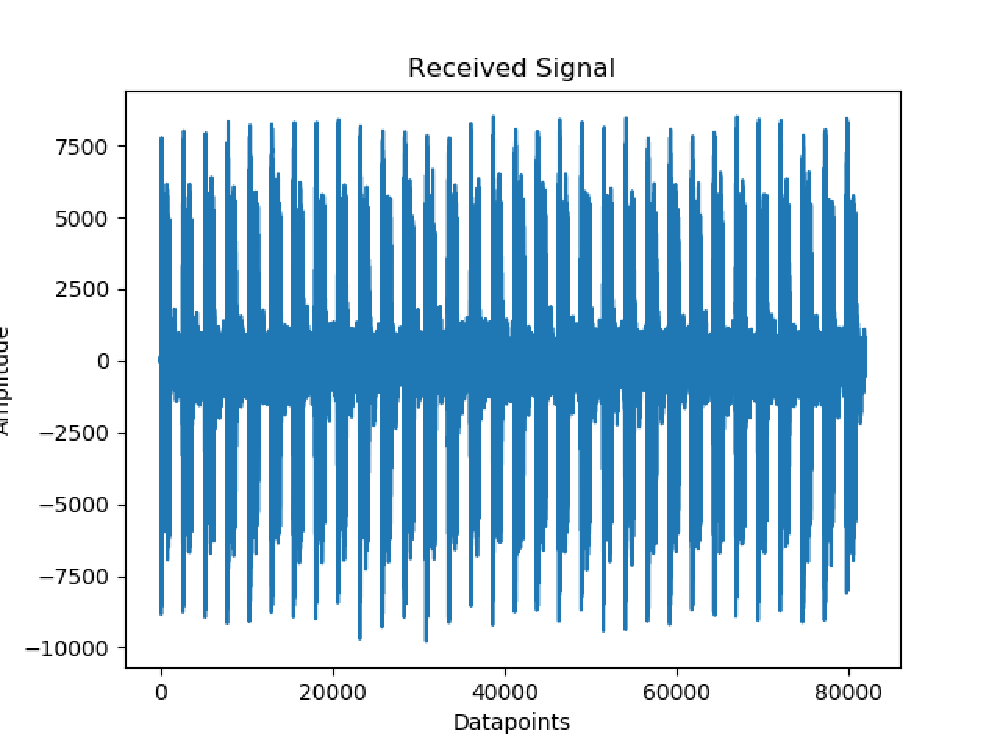
\includegraphics[width=0.9\textwidth]{images/rxSig.pdf}
        \caption{Received Signal}\label{fig:rxSignal101}
    \end{minipage}\hfill
    \begin{minipage}{0.45\textwidth}
        \centering
        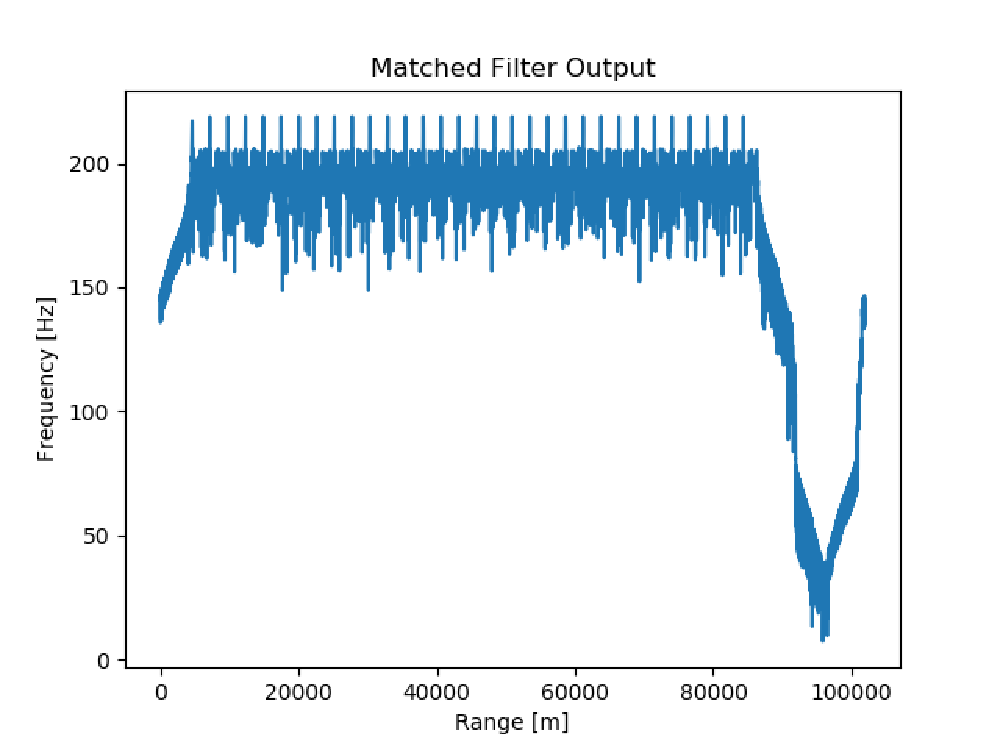
\includegraphics[width = 0.9\textwidth]{images/mf.pdf}
        \caption{Matched Filter Output}\label{fig:matchedfilterOutput}
    \end{minipage}
\end{figure}

\subsubsection{Range Line vs Time}
A range matrix follows the matched filter output as explained in Chapter \ref{chap:Radar Theory}. After obtaining the range matrix, the whole matrix undergoes a windowing function as explained in Section \ref{window}. In addition to windowing the matrix, the range matrix is also corrected for phase leakage that is introduced by the speaker and microphone playing and recording a sine wave. The first column of the range matrix is considered the $0^\circ$ datum that the other phases would be measured against. The phase (angle) of the first column is used to generate a complete matrix with the same dimensions as the range matrix duplicating the first column. The range matrix is then multiplied by the conjugate (to cancel the phase leakage) of the phase leakage matrix and also multiplied by the windowing function. The matrix also needs to undergo an FFT that needs to be applied in the slow time. This refers to the rows (or the number of pulses) of the matrix. The output of the slow time FFT applied to the matrix is the range map. 

The signal processing of the Pulsed-Doppler radar was executed and tested on a computer running MATLAB. The resultant range line from a test using real-world data can be seen in Figure \ref{fig:pdMATLAB} showing the successful implementation of the range map using a real speaker and microphone. The end result of the embedded radar would be compared to this result.

\begin{figure}[h!]
    \centering
    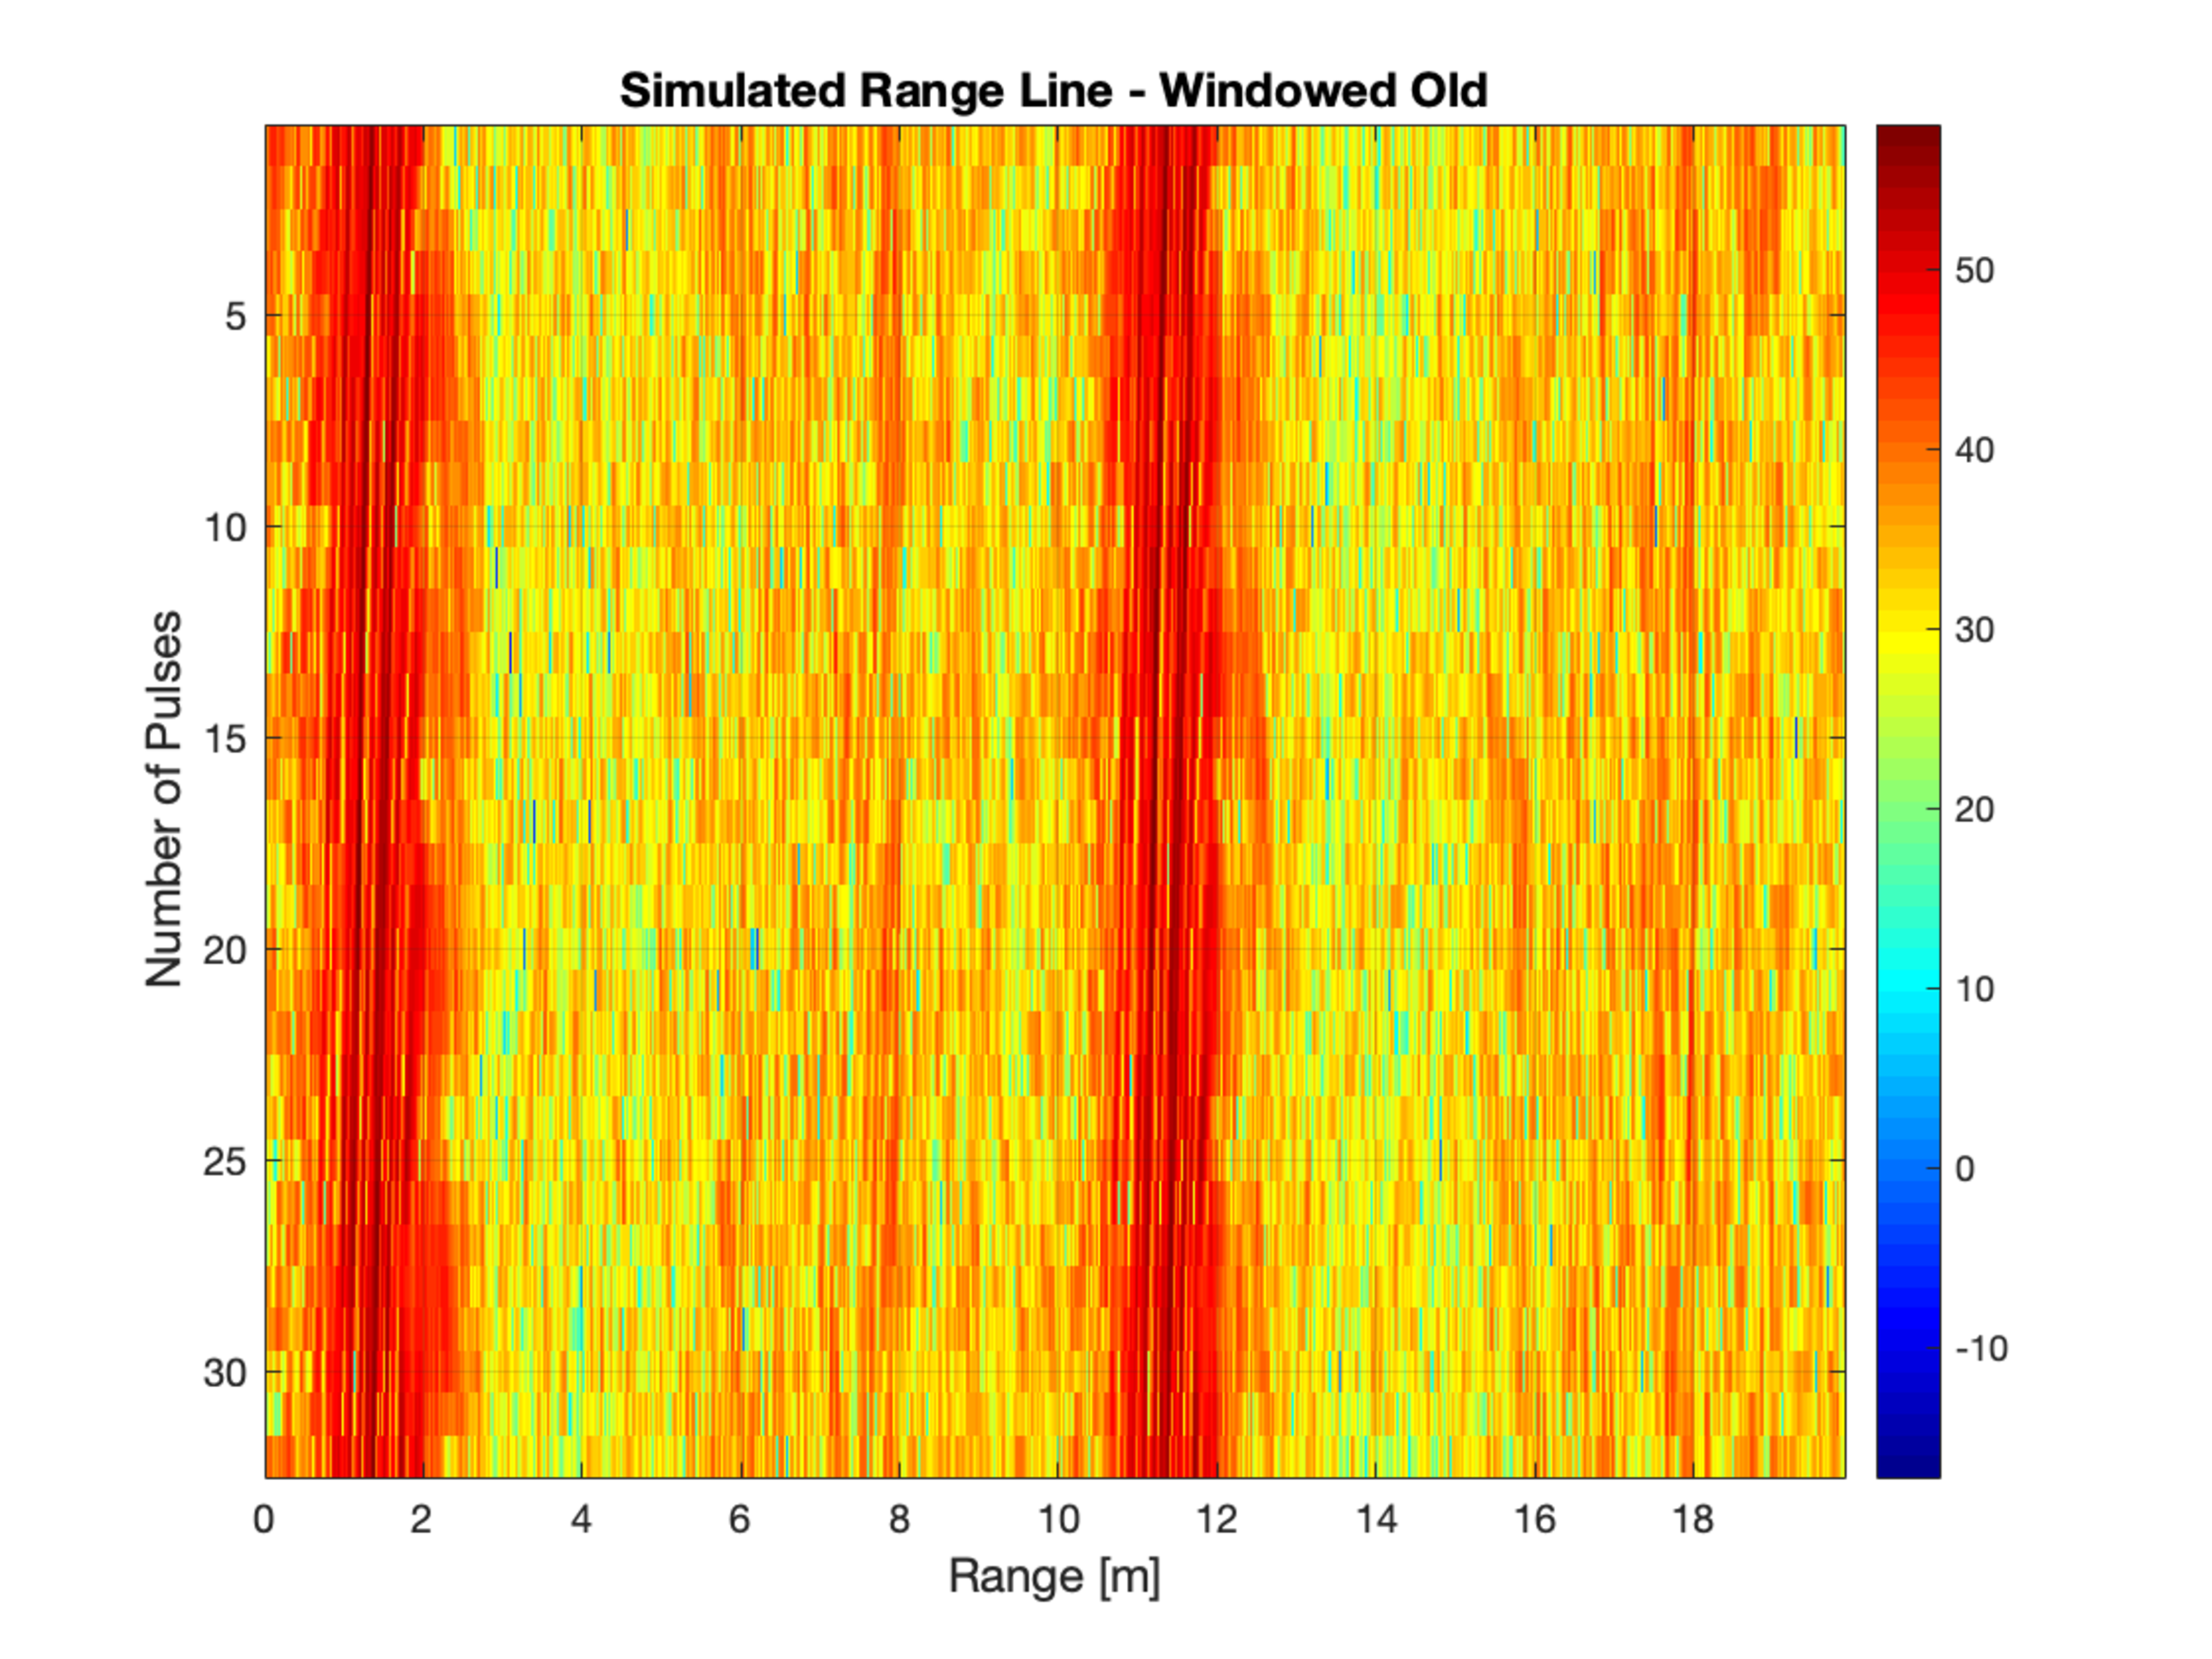
\includegraphics[width = 0.6\textwidth]{images/pd.pdf}
    \caption{Range Map from MATLAB}\label{fig:pdMATLAB}
\end{figure}

The function (in Python) that windows and gets rid of the phase leakage that the radar experiences, and FFT the matrix can be seen below. It takes in the received signal matrix and returns the windowed, phase leakage corrected matrix and FFTed matrix that is the range map.  %degree symbol

{\small\begin{verbatim}
def hamming(RxSignalMatrix):
        n = RxSignalMatrix.shape[0]
    m = RxSignalMatrix.shape[1]
    h = signal.hamming(n)
    Window = np.transpose(np.matlib.repmat(h, m, 1))
    phaseLeakageVector = np.angle(RxSignalMatrix[ : , 1])
    phaseLeakMatrix = np.transpose(np.matlib.repmat(phaseLeakageVector, m, 1))  
    RangeMatrix_Win_PhLeak = RxSignalMatrix * Window * np.conj(phaseLeakMatrix)
    RangeMatrix = fft(RangeMatrix_Win_PhLeak, axis=0) 
    return RangeMatrix 
\end{verbatim}}

Figure \ref{fig:rangemap} shows the applied range map as implemented on the radar system. The system was tested and the setup can be seen in Figure \ref{fig:setup}.

\begin{figure}[h!]
    \centering
    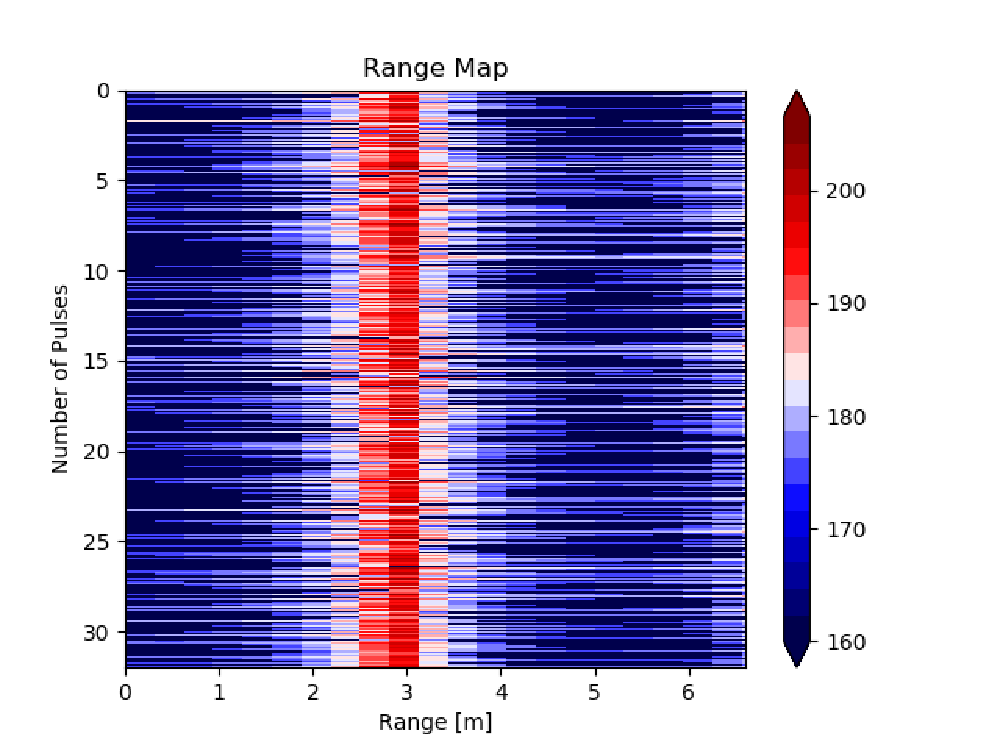
\includegraphics[width = 0.6\textwidth]{images/rangemap.pdf}
    \caption{Range Map}\label{fig:rangemap}
\end{figure}

\begin{figure}[h!]
    \centering
    {\begin{minipage}{0.45\textwidth}
        \centering
        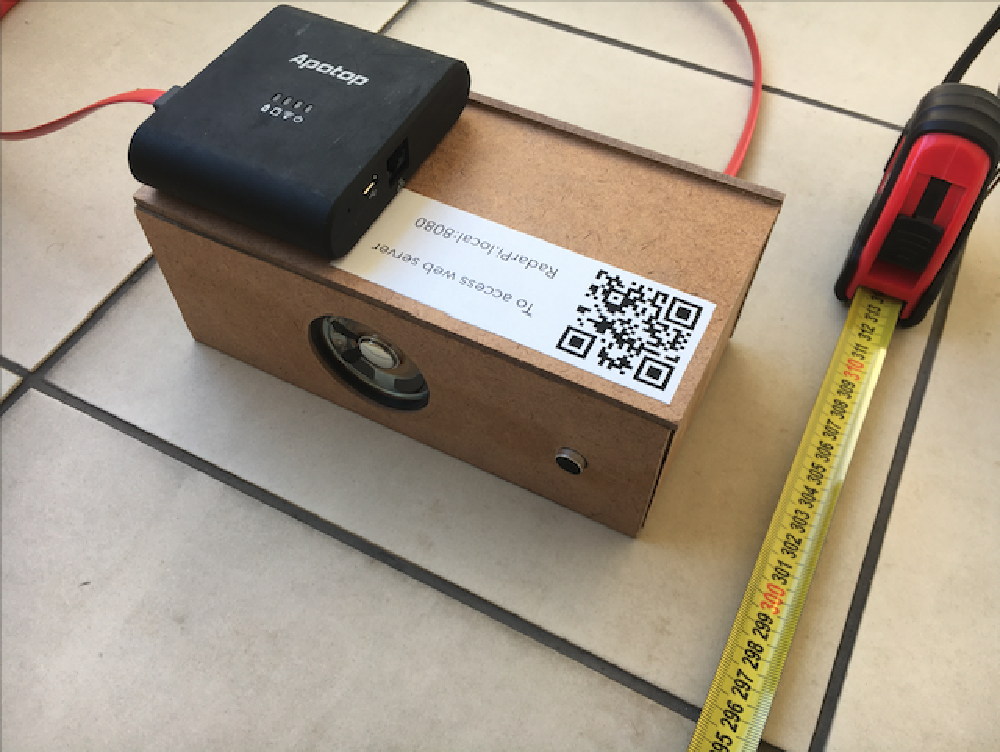
\includegraphics[width=0.9\textwidth]{images/test.pdf}
    \end{minipage}\hfill
    \begin{minipage}{0.45\textwidth}
        \centering
        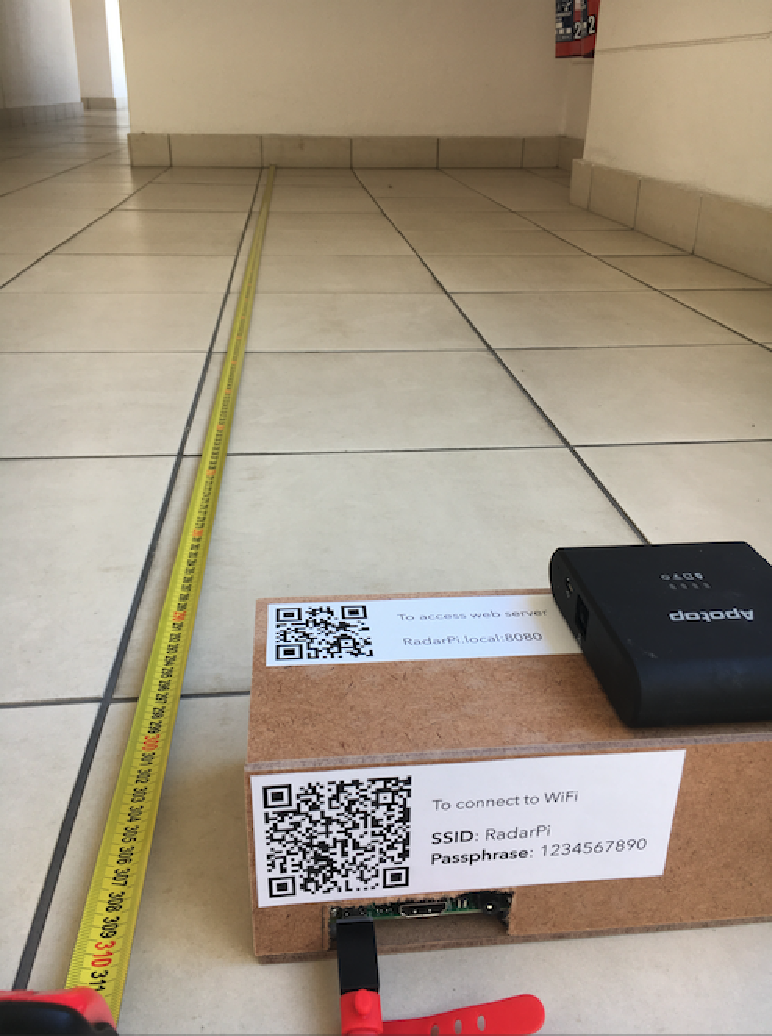
\includegraphics[width = 0.5\textwidth]{images/test1.pdf}
    \end{minipage}}\caption{Setup for Testing Range Map}\label{fig:setup}
\end{figure}

The radar was handheld to reduce the clutter from the floor. As seen in the figure, the wall registered at roughly $3\ m$ as was measured by the tape measure. The radar was powered by a power bank with a minimum power output of $7.5\ W$.

\subsection{Continuous Wave Radar Signal Processing and Implementation}
\subsubsection{Frequency variation and Doppler Effect}
The Continuous Wave radar implementation starts with generating a constant tone. The tone is generated using the Numpy package in Python and a sine function. The user would enter the duration of the tone to be played as well as the frequency. The function to generate the \verb wave  file can be seen below as implemented on the Raspberry Pi.

\small{\begin{verbatim}
def waveGenerator(duration, frequency=8000):
    fs = 44100
    t = np.linspace(0, duration, fs * duration) 
    y = np.int16(np.sin(frequency * 2 * np.pi * t) * 32767)
    path = "/home/pi/Documents/RadarPi"
    name = (os.path.join(path, "static", (str(int(frequency)) + 'Hz.wave'))) 
    wavfile.write(name, fs, y)
\end{verbatim}}

After the sound has been played (using the same function as the Pulse-Doppler radar) and recorded, the recorded signal undergoes a bandpass filter to get rid of static noises and clutter. The bandpass filter has cut-off frequencies $7.5\ \%$ lower and higher than that of the frequency on the tone generated. A bandpass filter lower- and higher cut-off frequencies for an $8000\ Hz$ tone would be $[7600,\ 8400]\ Hz$ respectively. The filter is designed every request by the radar with the \verb scipy.signal.firwin()  function and implemented using the \verb scipy.signal.convolve()  function.

\subsubsection{Spectrogram}

A spectrogram is a representation of the spectrum of frequencies in a signal. The matplotlib.pyplot package is used to generate the spectrogram by running the following code.
\small{\begin{verbatim}
Pxx, freqs, bins, im = plt.specgram(y, NFFT=16384, Fs=fs, noverlap=8092)
\end{verbatim}}
The \verb Pxx  is the power spectral density, \verb freqs  is the spectrum of frequencies, \verb bins  is the amount time that has passed, and \verb im  is the image file. Figure \ref{fig:cwSpec} shows the entire spectrum after the bandpass filter has been applied. \verb NFFT  is the number of slow time FFTs that are being done by the function to form the spectrogram. The frequency resolution depends on it. \verb noverlap  is the time resolution of the spectrogram. Figure \ref{fig:cwSpec1} shows the zoomed-in version of the same spectrogram centred around the tone frequency. It is visible to see that the recorded sound features the tone frequency. 

\begin{figure}[h!]
    \centering
    \begin{minipage}{0.45\textwidth}
        \centering
        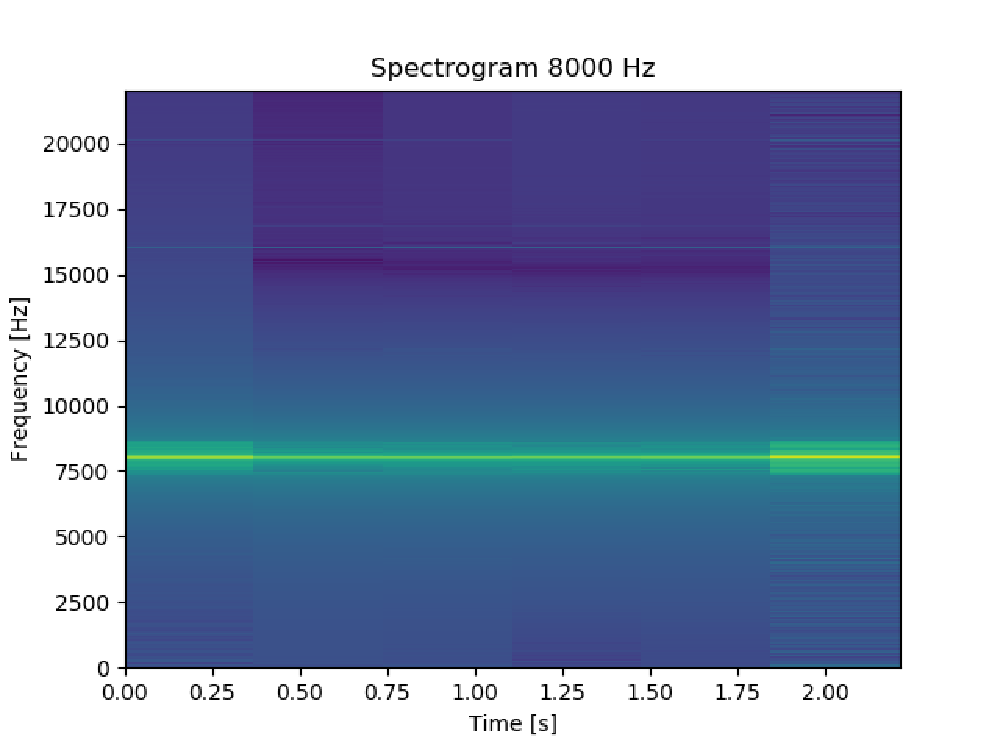
\includegraphics[width=0.95\textwidth]{images/cwSpec.pdf}
        \caption{Spectrogram Displaying All Registered Frequencies}\label{fig:cwSpec}
    \end{minipage}\hfill
    \begin{minipage}{0.45\textwidth}
        \centering
        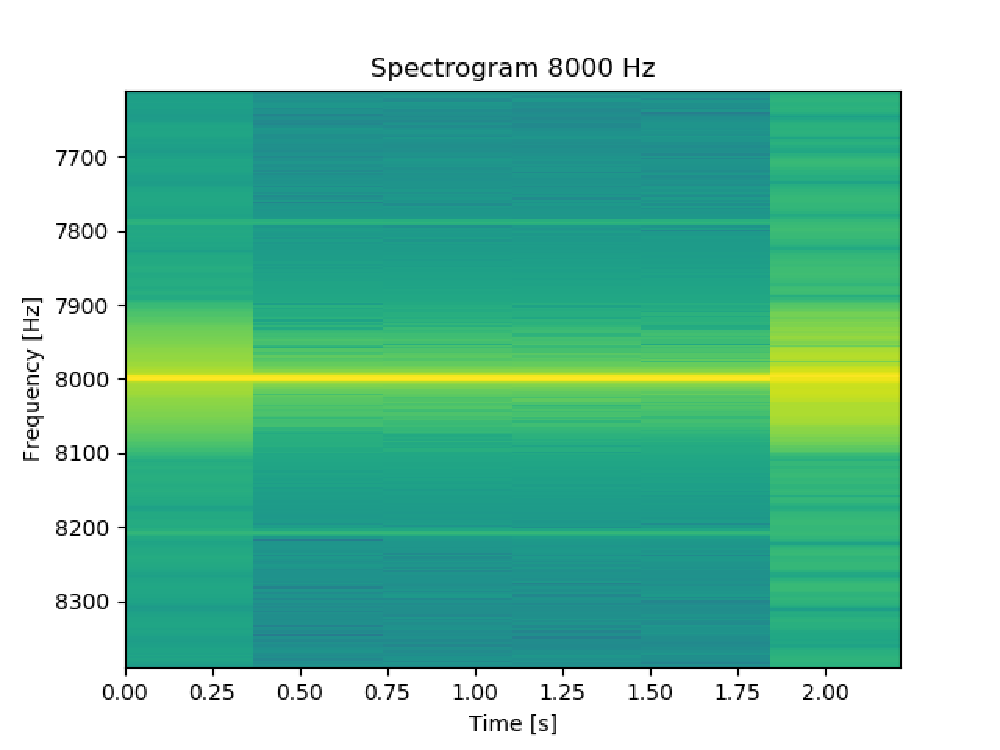
\includegraphics[width = 0.95\textwidth]{images/cwSpec1.pdf}
        \caption{Spectrogram Displaying Only Around Tone Frequency}\label{fig:cwSpec1}
    \end{minipage}
\end{figure}
The implemented spectrogram in the radar features a notch filter to get rid of the stationary clutter contained in the received signal. It is not the prospect of the CW radar to display the tone frequency but rather display any Doppler Frequencies recorded by the microphone. This Doppler Frequency represents the target moving. If no movement is detected, only the tone frequency would exist and that is not desirable. Figure \ref{fig:notchApplied} shows a box moving toward the radar with the notch filter applied. It is important to note that the ambient noises are amplified and with the filters applied, softer noises register more profoundly on the scale and are, therefore, more pronounced.

\begin{figure}[h!]
    \centering
    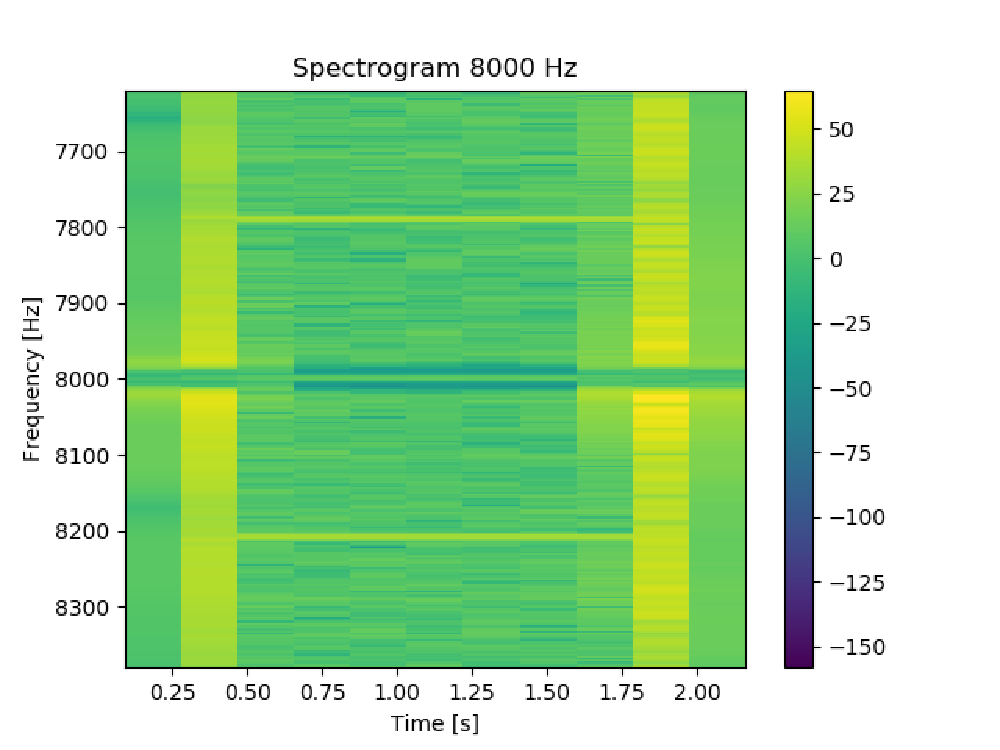
\includegraphics[width = 0.6\textwidth]{images/notchApplied.pdf}
    \caption{Spectrogram with notch filter applied and no movement.}\label{fig:notchApplied}
\end{figure}

The frequency as seen in Figure \ref{fig:notchApplied} in the third bin is a higher frequency than that of the played tone of $8000\ Hz$ indicating that the box is moving toward the radar. The observed frequency is roughly $8030\ Hz$ and using Equation \ref{eq:dopplerEffect}, the velocity is approximately:

\begin{equation}
8030 = \frac{343}{343-v_s}(8000)\\
v_s = 1.28\ m.s^{-1}
\end{equation}
\section{Implementation of Chosen Hardware Designs}
Using all of the chosen subsystems selected above, the following implementation of the design was chosen and can be seen in Figure \ref{fig:implementationCircuit}.

\begin{figure}[h!]
    \centering
    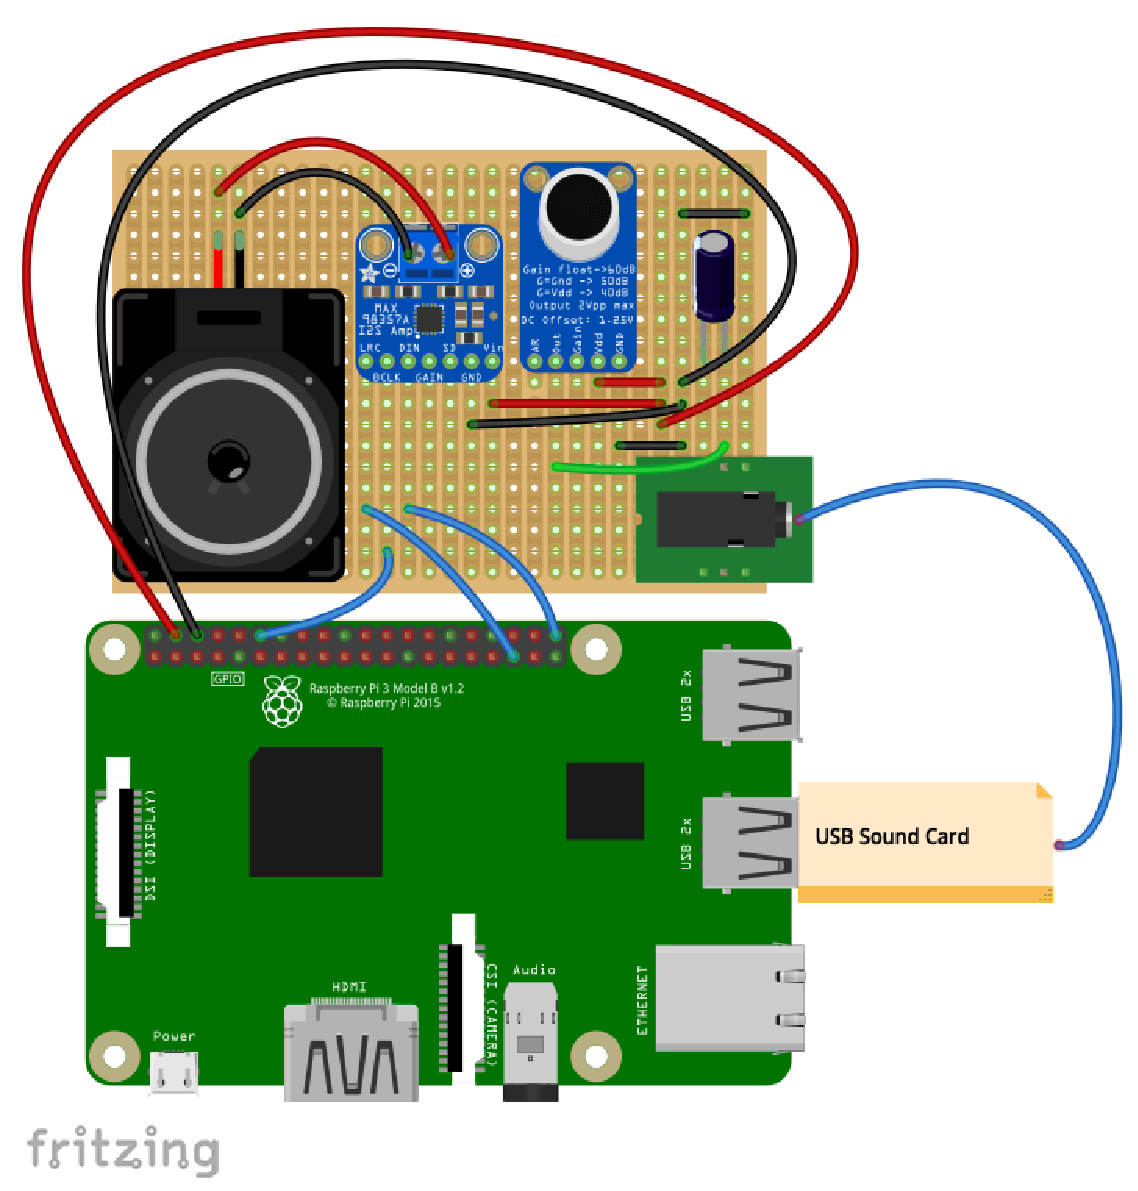
\includegraphics[width = 0.75\textwidth]{images/implementationCircuit.pdf}
    \caption{Enclosure with components visible}\label{fig:implementationCircuit}
\end{figure}

It can be seen that the MAX98357A module is connected to the $I^2S$ pins hosted on the Raspberry Pi 3B and directly driving the speaker. On the receiving side, the MAX9814 is connected to a $3.5\ mm$ audio socket that connects to the USB sound card. A capacitor is added to the $OUT$ pin of the microphone to act as a filter and block any $DC$ current to flow. This allows for the input to the sound card to only see the changes in voltage as generated by the microphone. The Veroboard designed to accommodate this circuit can be seen implemented in Figure \ref{fig:veroboard}.

\begin{figure}[h!]
    \centering
    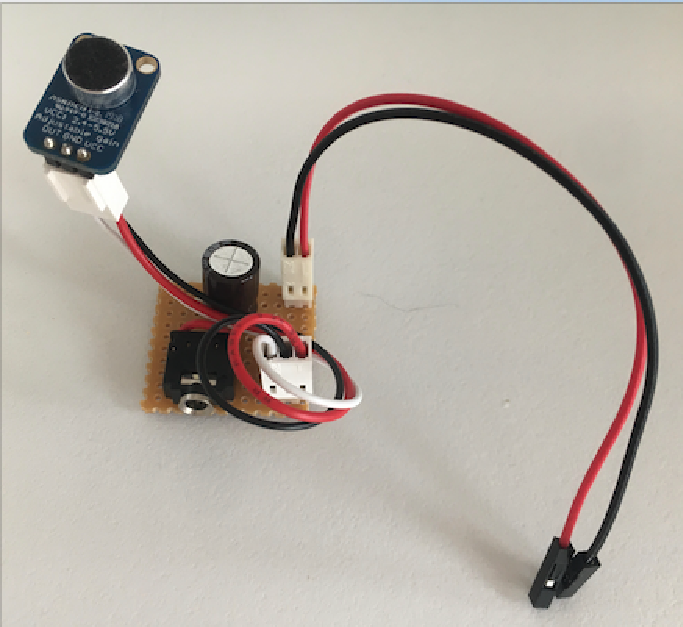
\includegraphics[width = 0.3375\textwidth]{images/veroboard.pdf}
    \caption{Veroboard implementation of microphone and $3.5\ mm$ socket}\label{fig:veroboard}
\end{figure}

Figures \ref{fig:enc3}, \ref{fig:enc1}, and \ref{fig:enc2} show the practical implementation with the manufactured enclosure as designed in Section \ref{enclosureDesign} combined with the circuitry layout from above. The enclosure was made using medium-density fibreboard (MDF) to add structural integrity and also protection from the outside world. The cost of the MDF amounted to $R\ 50.00$ which included two A4 sheets. 

\begin{figure}[h!]
    \centering
    \begin{minipage}{0.45\textwidth}
        \centering
        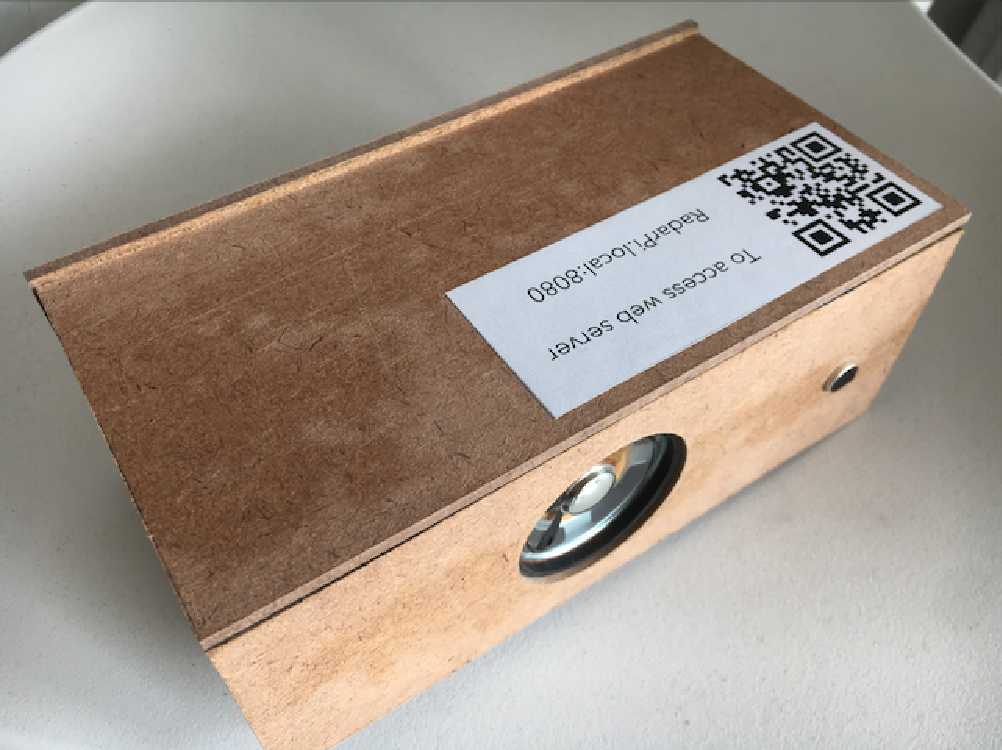
\includegraphics[width = 0.75\textwidth]{images/enc3.pdf}
        \caption{Front Facing View of Enclosure}\label{fig:enc3}
    \end{minipage}\hfill
    \begin{minipage}{0.45\textwidth}
        \centering
        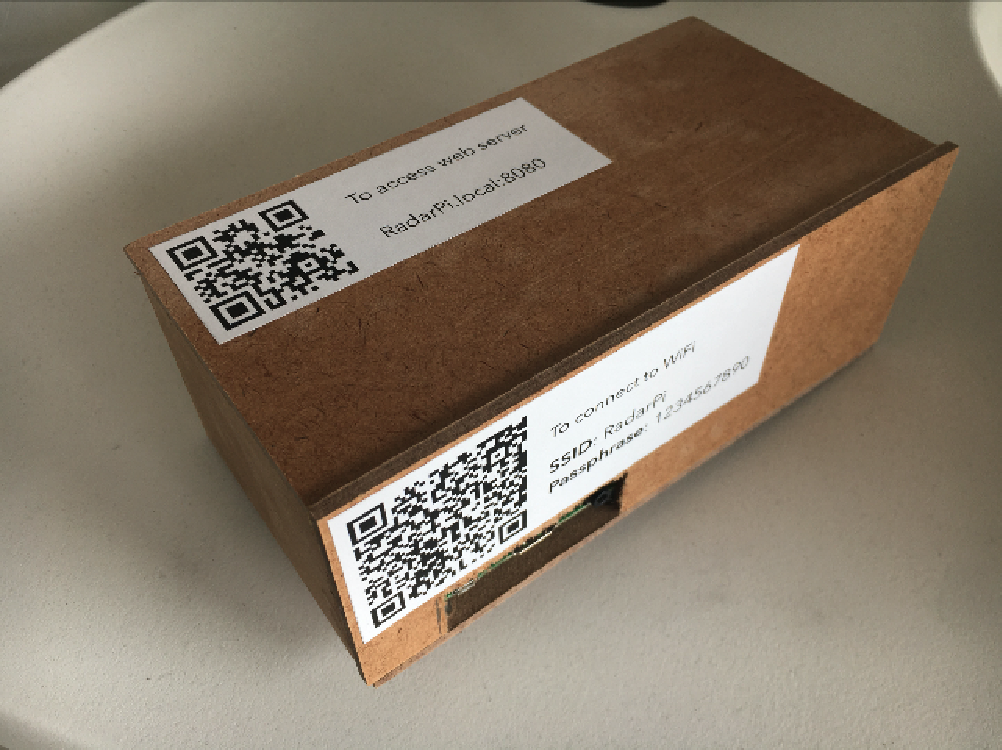
\includegraphics[width=0.9\textwidth]{images/enc1.pdf}
        \caption{Rear Facing View of Enclosure}\label{fig:enc1}
    \end{minipage}
\end{figure}

\begin{figure}[h!]
    \centering
    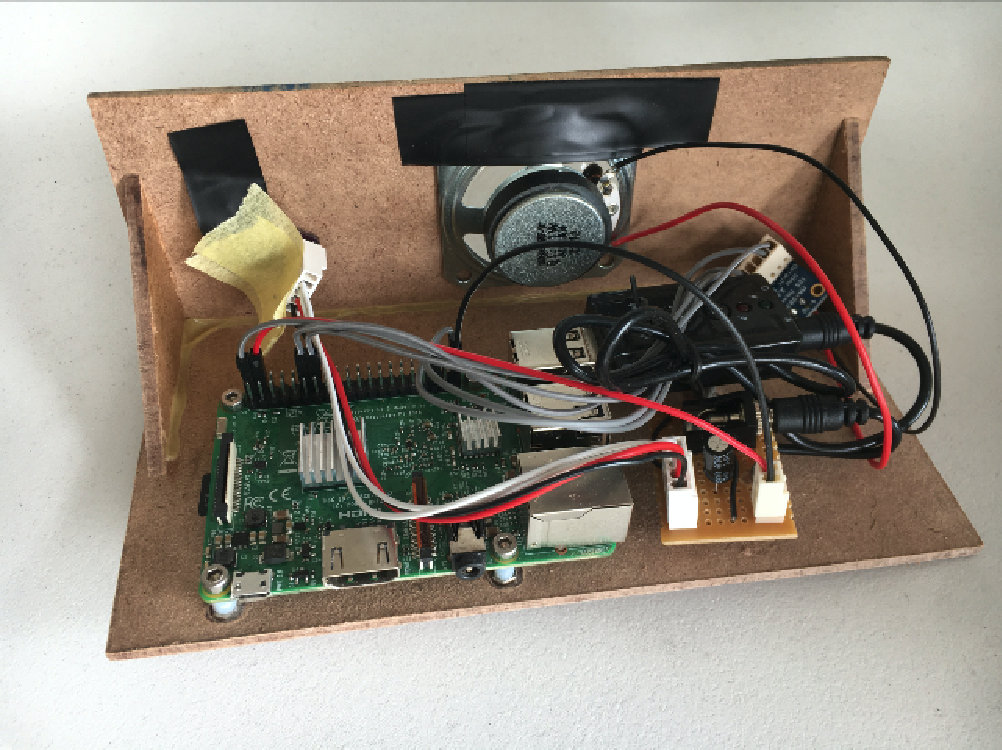
\includegraphics[width = 0.3375\textwidth]{images/enc2.pdf}
    \caption{Rear Facing View of Enclosure (Open)}\label{fig:enc2}
\end{figure}

The QR-codes on the enclosure is for connecting to the Wi-Fi as broadcast by the Raspberry Pi and for a quick link to visit the web page hosted on the Raspberry Pi. From the web page, all of the parameters for both methods of detection can be set and the results displayed.

\section{Energy Budget}
The following energy budget has been set up as the 'worst-case' possible for all of the components. The table can be seen in Table \ref{table:energyBudget}.

\begin{table}[h!]
\centering
\begin{tabular}{lll}
\hline
\textbf{Item} & \textbf{Criteria} & \textbf{Energy Consumption} \\ \hline
\\ \textbf{Raspberry Pi 3B} & 400\% CPU & 730 mA \\
\\ \textbf{$I^2S$ DAC} & Playing at highest volume & 360 mA \\
\\ \textbf{Speaker} & Playing at highest volume & 200 mA \\
\\ \textbf{USB Sound Card} & Only recording & 110 mA \\
\\ \textbf{Microphone} & \begin{tabular}[c]{@{}l@{}}Quiet environment\\ (maximum gain)\end{tabular} & 105 mA \\ \\ \hline
 &  & 1505 mA  Total\\ \cline{3-3}
\end{tabular} \caption{Energy Budget}\label{table:energyBudget}
\end{table}

\newpage